% -
\chapter{Precipitación total}\label{cap:resultados_tp}
% -

% ==============================================================================
% SECCIÓN PRINCIPAL: PDF DE PRECIPITACIÓN TOTAL
% ==============================================================================

\section{Distribución de magnitudes (PDF)}\label{sec:pdf_tp}

\begin{figure}[htbp]
\centering
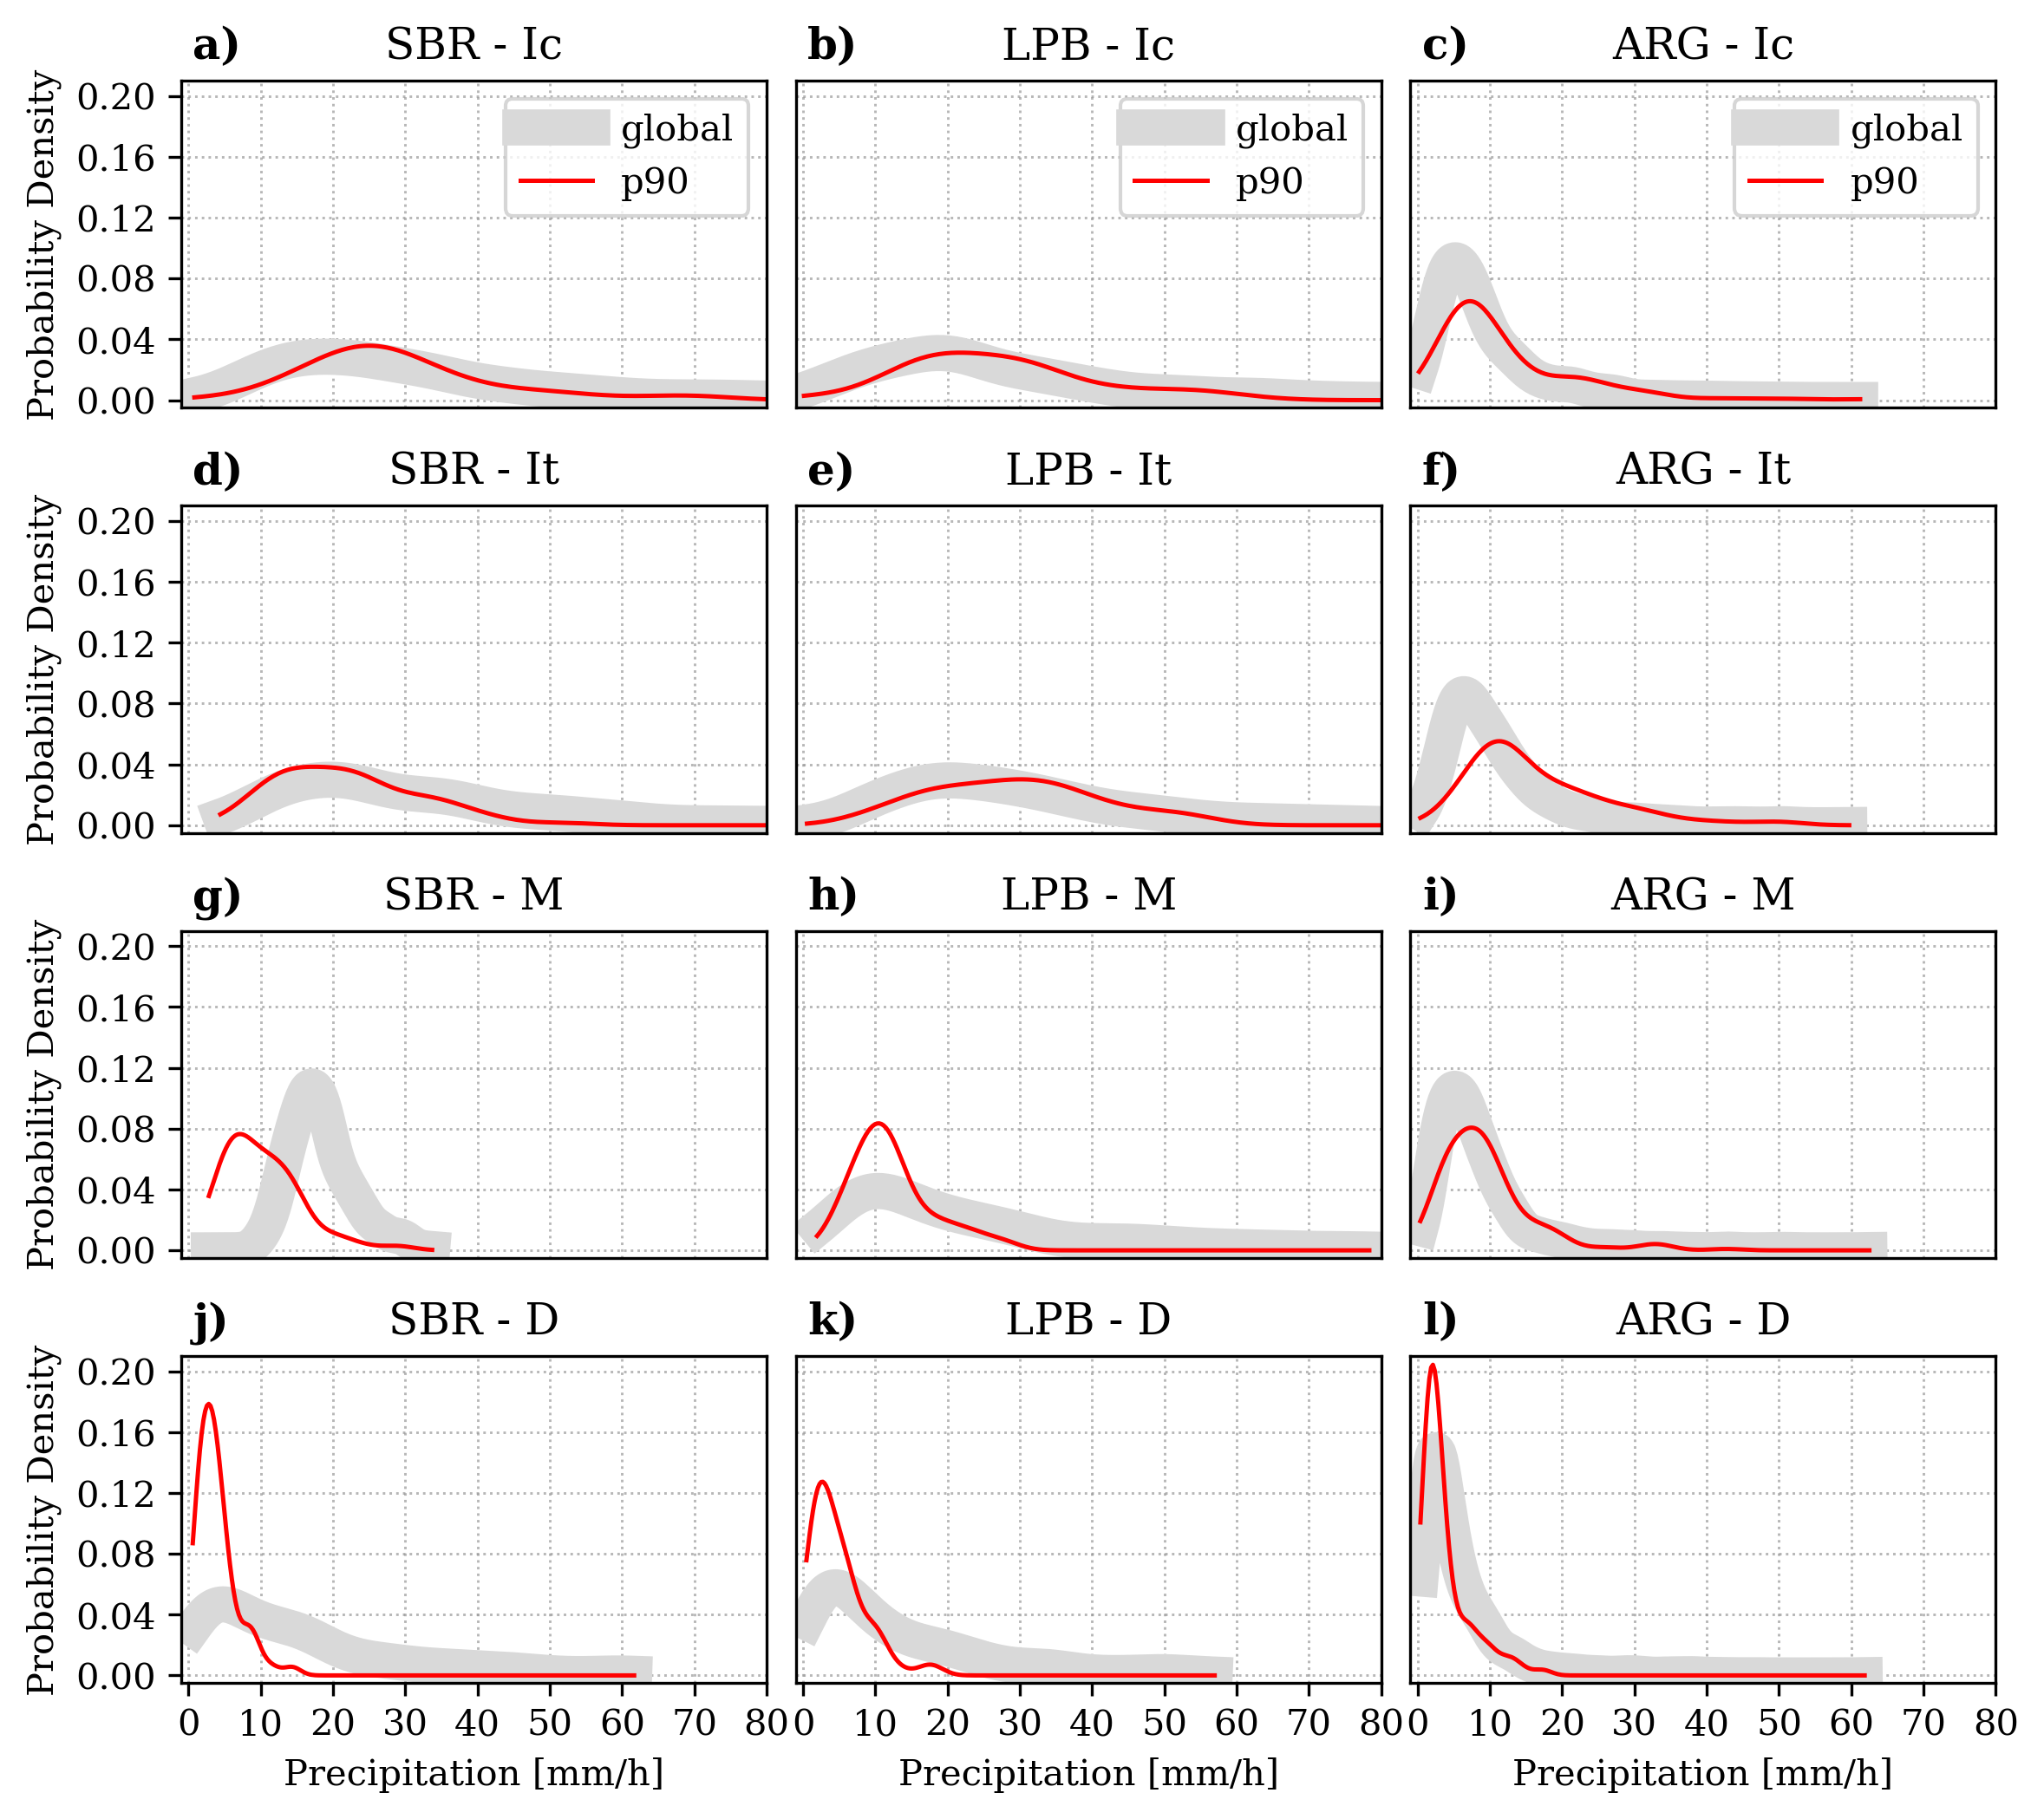
\includegraphics[width=\textwidth]{images/tp/PDF_tp_sigma025.png}
\caption[PDF de magnitudes máximas de precipitación total]{Funciones de densidad de probabilidad (PDF) para las magnitudes máximas de precipitación total (mm/h). Las columnas indican la región de ciclogénesis (SBR, LPB, ARG) y las filas la evolución a través de las fases del ciclo de vida (Ic, It, M, D). Se contrasta la población global (referencia, sombreado gris) con el subconjunto de los máximos de vorticidad relativa en 850 hPa alcanzados en su ciclo de vida: p90 (sistemas extremos, linea roja).}
\label{fig:pdf_tp}
\end{figure}

La Figura~\ref{fig:pdf_tp} muestra la distribución estadística de los máximos espaciales de precipitación total (mm/h). Estos campos fueron extraídos sistemáticamente dentro del dominio lagrangiano de $20^\circ \times 20^\circ$ centrado en el núcleo de cada sistema, siguiendo la misma metodología aplicada al campo de viento (Capítulo~\ref{cap:resultados_wind10}). La Población global se encuentra estratificada por región de ciclogénesis (SBR, LPB, ARG) y el subconjunto de intensidad dinámica definido según el pico máximo absoluto de vorticidad alcanzado durante todo el ciclo de vida de cada ciclón eventos extremos (p90).

En las fases de incipiencia e intensificación (paneles a-f), SBR y LPB muestran distribuciones anchas donde los ciclones extremos (p90) presentan una marcada tendencia hacia mayores tasas de precipitación, con colas que se extienden hasta los 60 mm/h. Como detallan \citet{chen2024evaluation}, la precipitación total resulta de la suma de la precipitación estratiforme a gran escala y la precipitación convectiva parametrizada, siendo esta última la que controla específicamente la cola superior de la distribución. En entornos con mayor disponibilidad de humedad e inestabilidad estática como los que caracterizan a SBR y LPB, el desarrollo de los ciclones más intensos está intrínsecamente ligado a una mayor actividad convectiva \citep{sinclair2023relationship}. A su vez, esta convección genera forzantes diabáticos que, como demuestran \citet{oertel2021warm} y \citet{blanchard2021warm}, propician las tasas de precipitación de alta intensidad a corto plazo responsables de engrosar el percentil superior (p90) durante las fases de desarrollo.

Sin embargo, al alcanzar la fase de madurez (paneles g-h) y profundizarse hacia el decaimiento (paneles j-k), ocurre una divergencia estructural: la curva del estrato p90 en SBR y LPB colapsa hacia la izquierda, desarrollando un pico modal sumamente estrecho en valores mínimos de precipitación (entre 1 y 4 mm/h). Simultáneamente, la Población Global retienen distribuciones mucho más extendidas y pluviosas centradas entre los 15 y 20 mm/h. Por su parte, la región de ARG (paneles c, f, i, l) manifiesta un régimen independiente donde las distribuciones permanecen en su mayor parte fuertemente sesgadas hacia magnitudes bajas (moda en $\sim$5 mm/h), destacándose una dispersión ligeramente mayor para el p90 durante la intensificación y, en el decaimiento (panel l), un colapso modal del estrato p90 hacia valores mínimos ($\sim$2--3 mm/h) análogo, aunque de menor magnitud, al observado en SBR y LPB.

La disparidad en las colas pluviométricas revela forzantes ambientales regionales distintos. Como demuestran \citet{russo2025impacts}, SBR y el límite con LPB presentan flujos de calor oceánico que sostienen la baroclinicidad y anclan la convección profunda en los sistemas extratropicales. Este ensanchamiento estadístico de la precipitación en la pobalcion global se acentúa por la presencia anual de ciclones subtropicales alimentados por estas mismas anomalías térmicas \citep{evans2012climatology}. Dinámicamente, esta energía convectiva que aporta al estrato extremo (p90) se organiza mediante una fuerte advección cálida y convergencia de humedad: impulsada por la Alta Subtropical en SBR, y por su interacción con el Chorro de Capas Bajas en LPB \citep{gramcianinov2024early}. En contraste, ARG presenta precipitaciones marcadamente menores, reflejando un forzamiento de latitudes altas caracterizado por baja humedad absoluta y advecciones frías y secas provenientes del Pacífico sur.
%%
La asimetría en las distribuciones pluviométricas refleja directamente las condiciones del entorno de génesis. Como señalan \citet{gramcianinov2019properties}, los ciclones originados en ARG están dominados por la baroclinicidad de latitudes medias, mientras que en LPB y SBR dependen fuertemente de la liberación de calor latente. Desde la energética atmosférica, \citet{coutodesouza2024thesis} corrobora esta dualidad al demostrar que los sistemas en ARG se sustentan en la cadena baroclínica clásica, en contraste con LPB y SBR, impulsados activamente por la cadena baroclínica húmeda de origen convectivo. Esta marcada diferencia en la disponibilidad de humedad y el forzamiento diabático es lo que explica físicamente el sesgo positivo y las mayores tasas de precipitación observadas en estas regiones.
% 

El desacople entre la máxima intensidad dinámica y la máxima precipitación durante la madurez confirma la relación no lineal entre la vorticidad y los forzantes de la precipitacion. Desde una perspectiva física, este comportamiento revela que los vórtices extremos (p90) evolucionan estructuralmente hacia sistemas profundos. Al alcanzar su máximo, estos ciclones severos agotan su acceso a la masa de aire húmedo e inestable transportada por la cinta transportadora cálida (\textit{warm conveyor belt}), la cual es responsable de la convección embebida más intensa \citep{oertel2021warm, blanchard2021warm}. En su lugar, el núcleo experimenta una pronunciada intrusión seca (\textit{dry intrusion}) inducida por la fractura frontal, un proceso mediante el cual aire frío, subsidente y de baja humedad proveniente de la alta troposfera o estratosfera se enrosca hacia el centro del sistema \citep{shapiro1999bridge}. Esta dinámica suprime drásticamente la convección profunda en el dominio central. 
% Por el contrario, los sistemas moderados (p50), al no ocluirse de forma tan violenta o prematura, logran sostener una interacción baroclínica. 
Este comportamiento termodinámico a lo largo del ciclo de vida complementa la caracterización espacial de \citet{gramcianinov2019properties}, quienes confirman que, los ciclones originados en SBR y LPB concentran las tasas de precipitación más intensas con una marcada similitud entre ambas regiones, mientras que los sistemas de ARG exhiben una naturaleza inherentemente más seca, registrando una menor cantidad de eventos que superen los 20 mm/día.
%%

La relación entre la vorticidad en 850 hPa del ciclón y los volúmenes máximos de precipitación exhibe un comportamiento no lineal. Al evaluar múltiples medidas de intensidad, \citet{corner2025classification} evidencian que las tasas pluviométricas se correlacionan moderadamente con la vorticidad en 850 hPa debido a mecanismos de retroalimentación donde el calentamiento diabático asociado a la lluvia intensa genera anomalías de vorticidad potencial que refuerzan la circulación en niveles bajos. Esta eficiencia termodinámica sustenta las colas pesadas de precipitación (superiores a 60 mm/h) observadas en las PDF del estrato p90 para SBR y LPB durante las etapas de intensificación, antes de que el aislamiento del núcleo corte el suministro de humedad.

La cuantificación de este comportamiento estadístico invertido permite refutar empíricamente la hipótesis de que la severidad del forzamiento dinámico (vorticidad máxima) se traduce invariablemente en un incremento de la lluvia extrema a lo largo de todo el ciclo de vida. Demostrar que, en el Atlántico Sur, los ciclones responsables de los vientos más destructivos tienden a secarse en su núcleo durante la madurez. Las amenazas más severas por lluvias asociadas a ciclones intensos (p90) ocurrirán predominantemente durante las etapas tempranas de génesis (incipiente) e intensificación, o bien estarán asociadas a sistemas de intensidad rotacional moderada cuyas configuraciones termodinámicas son más eficientes para sostener el anclaje convectivo prolongado.

% ==============================================================================
% SECCIÓN PRINCIPAL: KDE ESPACIAL DE PRECIPITACIÓN
% ==============================================================================

\section{Distribución espacial de máximos (KDE)}

\subsection{Población Global}\label{subsec:kde_tp_global}

\begin{figure}[htbp]
\centering
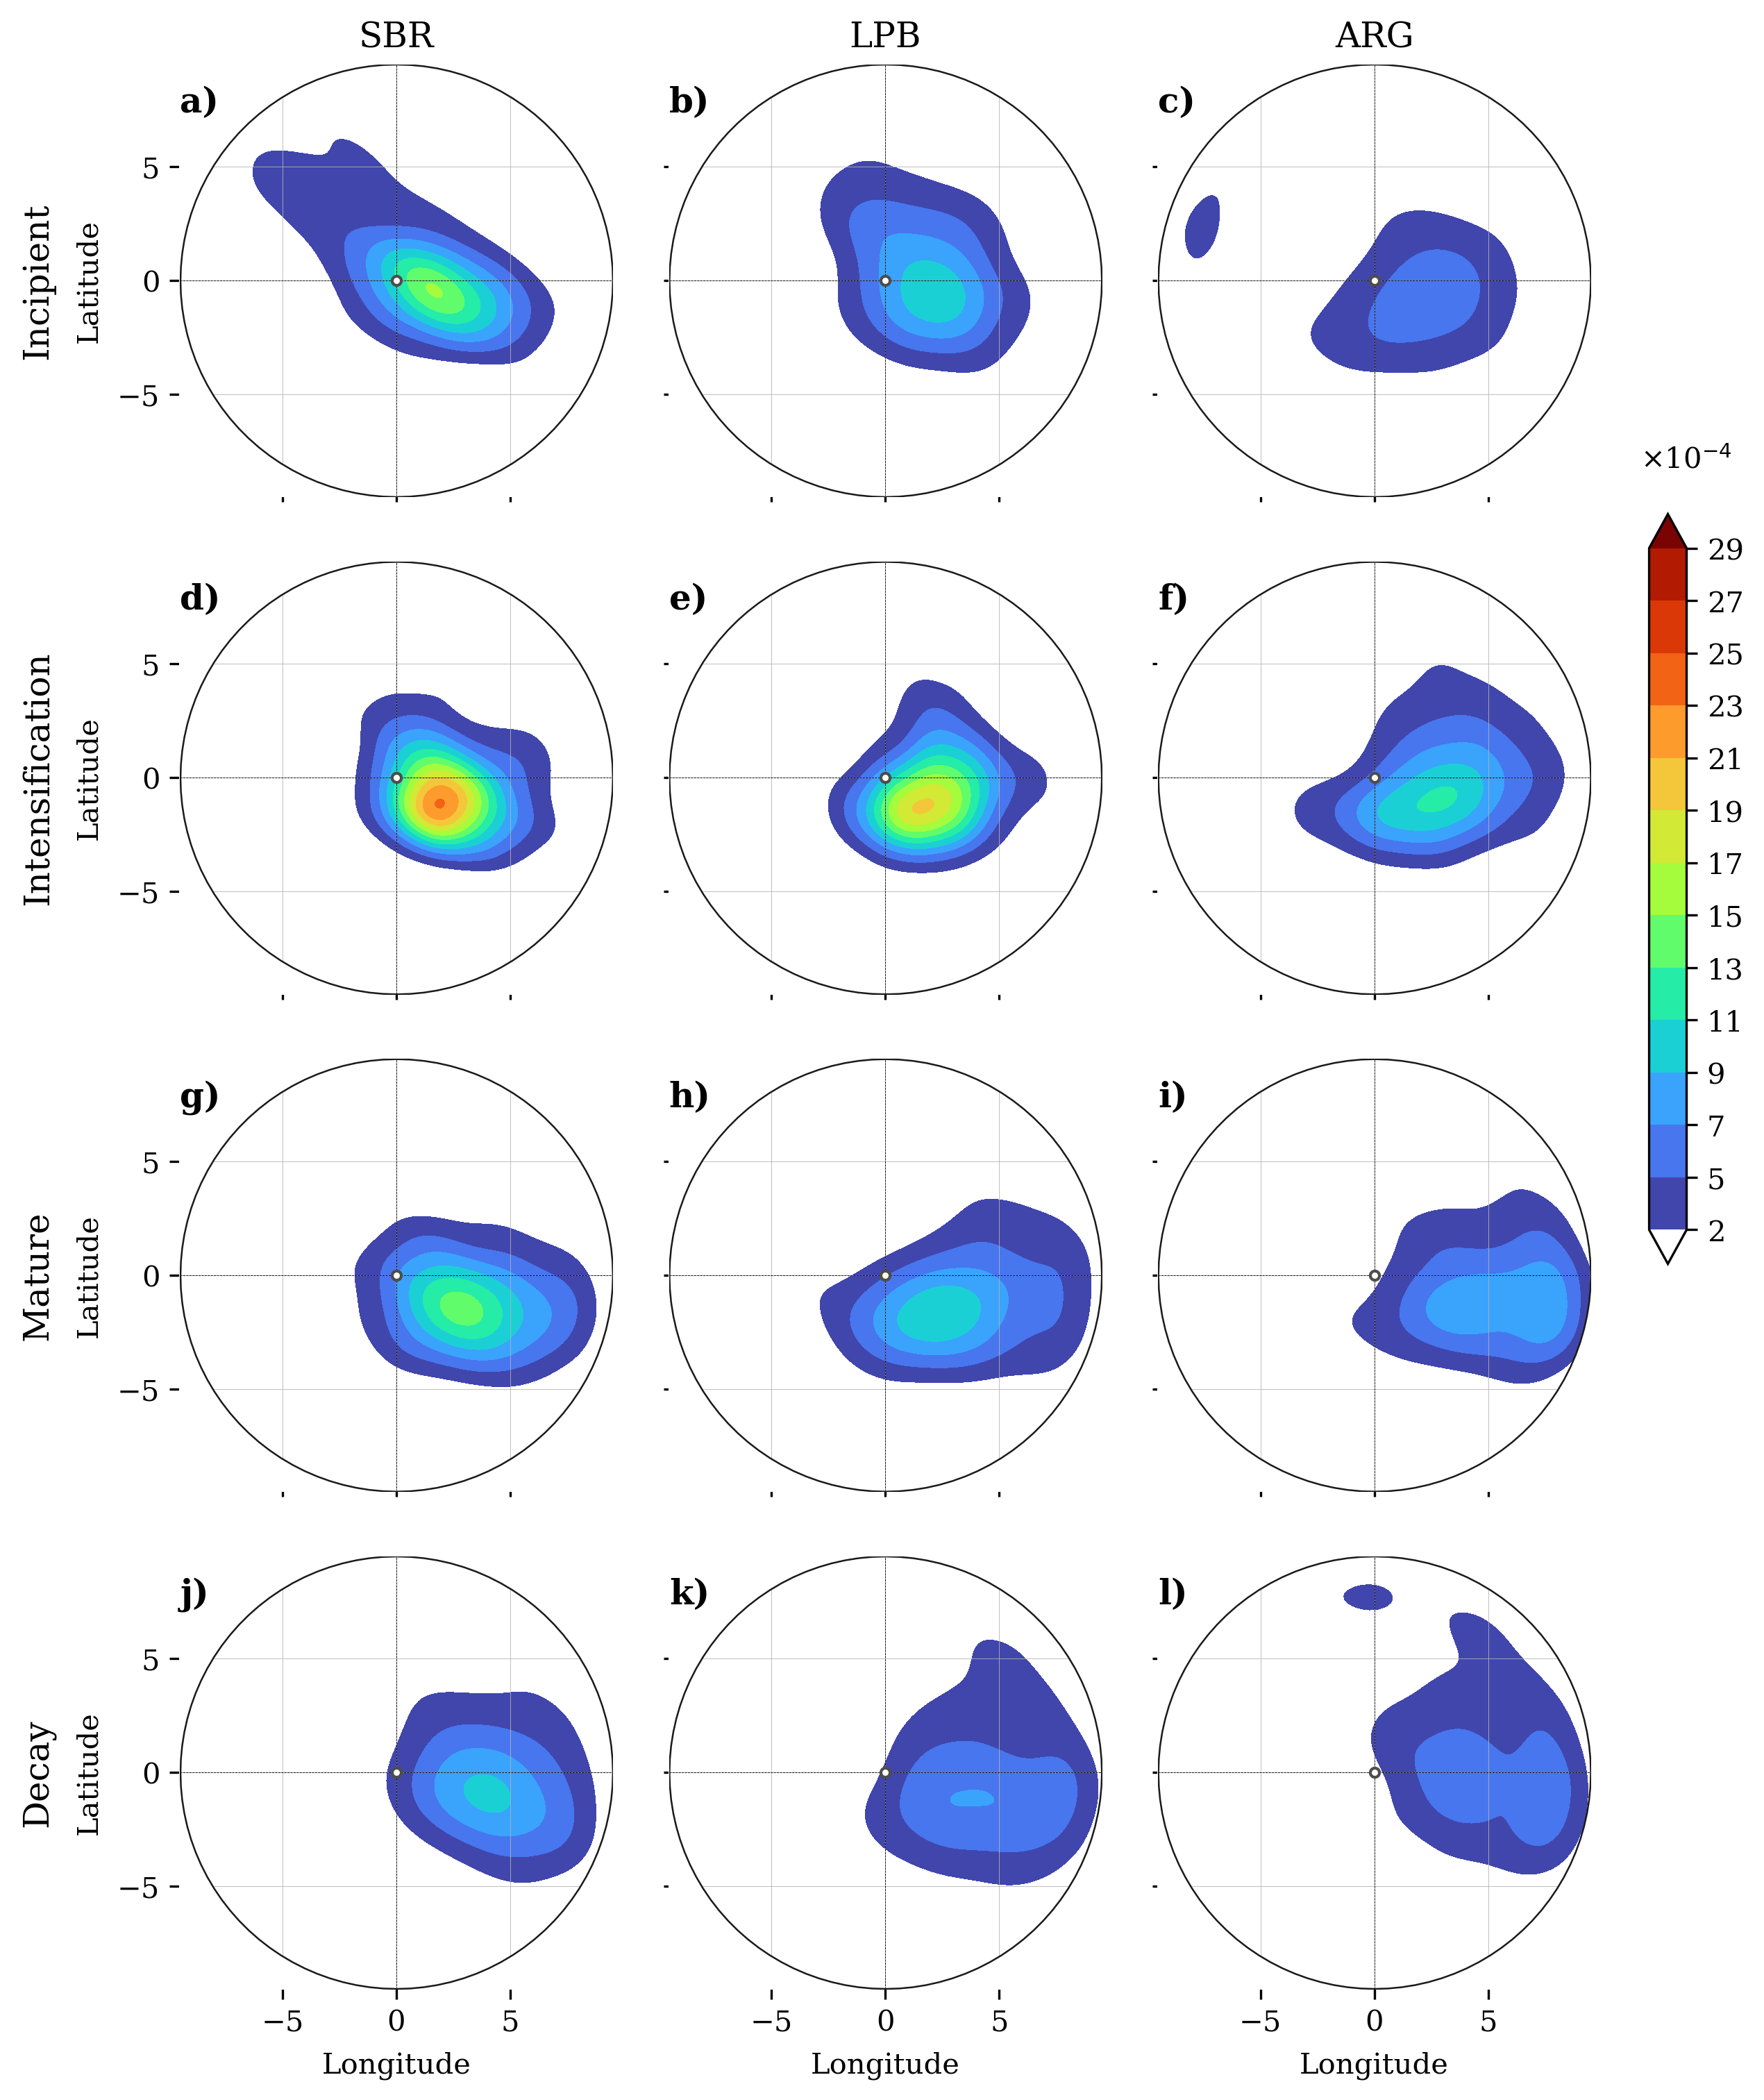
\includegraphics[width=\textwidth]{images/tp/kde_tp_global_fasesxreg.png}
\caption[Distribución espacial (KDE) de precipitación máxima - Población Global]{Estimación de densidad espacial bidimensional (KDE) para la ubicación geométrica de los máximos de precipitación total (mm/h) en la Población Global de referencia. La matriz organiza la evolución espacial a través de las fases evolutivas Incipiente (a-c), Intensificación (d-f), Madurez (g-i) y Decaimiento (j-l), segregadas por las regiones de ciclogénesis SBR, LPB y ARG. El dominio lagrangiano abarca $20^{\circ} \times 20^{\circ}$ con centro en el vórtice $(0,0)$. La barra de colores cuantifica la densidad de probabilidad relativa escalada por $10^{-4}$.}
\label{fig:kde_tp_global}
\end{figure}

La Figura~\ref{fig:kde_tp_global} presenta el campo probabilístico derivado de la estimación de densidad por kernel (KDE), el cual mapea la ubicación espacial preferencial de los núcleos de precipitación máxima para la Población Global dentro del marco de referencia lagrangiano. A diferencia del campo de viento cuya distribución incipiente ya evidenciaba cierta difusión centrada en el núcleo, la distribución espacial de la lluvia máxima presenta desde las etapas iniciales una arquitectura fundamentalmente asimétrica respecto al centro del ciclón.

La asimetría hacia el sector oriental y sureste observada en el KDE de la Población Global (Fig.~\ref{fig:kde_tp_global}, paneles a-f) emerge primariamente de la arquitectura dinámica del Cinturón Transportador Cálido (WCB, \textit{Warm Conveyor Belt}). Según el modelo conceptual de \citet{browning1986conceptual} y las evaluaciones observacionales de \citet{naud2020evaluation}, el ascenso inclinado del WCB por delante del frente frío y por encima del frente cálido organiza la precipitación en el flanco cálido del ciclón, independientemente de la región de génesis. Este forzante sinóptico explica la carga positiva consistente del EOF1 en el cuadrante sureste (Fig.~\ref{fig:eof1_tp_global}) y constituye el esqueleto dinámico universal de la distribución espacial: en el Hemisferio Sur, las condiciones de ascenso a gran escala acoplado a advección de humedad se satisfacen casi exclusivamente en este sector. La orientación hacia el este y sureste de las densidades máximas en las fases incipiente e intensificación (paneles a-f) refleja directamente esta organización.

Sobre este esqueleto dinámico del WCB, operan secundariamente moduladores regionales que explican las diferencias de intensidad y extensión entre SBR, LPB y ARG. En SBR y LPB, la configuración de los flujos en la capa límite refuerza la asimetría oriental, como demuestran \citet{cardoso2022synoptic}, la circulación ciclónica induce anomalías positivas de convergencia de humedad acopladas con advección cálida en niveles bajos, organizando la precipitación en bandas orientadas de noroeste a sureste. Adicionalmente, el flujo canalizado desde latitudes tropicales hacia el flanco este del vórtice, documentado por \citet{vera2002cold}, actúan como focos de convergencia que intensifican la asimetría, resultando en núcleos de precipitación más densos y extendidos en el KDE (paneles a, b, d, e). En contraste, para ARG, la mayor distancia a la fuente de humedad tropical y la barrera orográfica de los Andes atenuan este flujo, generando un patrón más difuso, menos intenso y con máximos desplazados hacia el noreste (paneles c, f, i, l), donde la advección zonal modificada por la topografía impone una organización distinta.

La robustez estadística de este patrón asimétrico en la Población Global es decir, su aparición consistente a pesar de la variabilidad inter-sistémica se debe al contexto climatológico de génesis y tracks. La alta frecuencia de ciclogénesis en las inmediaciones del norte de Argentina, Uruguay y sur de Brasil, junto con el desplazamiento preferente hacia el sureste sobre el océano \citep{mendes2010climatology, simmonds2000mean}, asegura una muestra donde el WCB interactúa sistemáticamente con la configuración regional descrita. Este tránsito constante de sistemas frontales maduros, caracterizado por frentes de avance relativamente estables que barren LPB y ARG, genera la huella dinámica que captura el KDE espacial. No obstante, es crucial distinguir que este contexto climatológico no es un forzante físico directo de la asimetría en un evento individual, sino un condicionante estadístico que garantiza la representatividad del patrón WCB-dominado en la muestra global.
% % REVISAR
% Finalmente, de manera episódica y estacional, la interacción con la Zona de Convergencia del Atlántico Sur (SACZ) puede reforzar localmente la precipitación oriental en SBR durante el verano austral \citep{hoskins2005new}. Sin embargo, su efecto es secundario y no altera la estructura media anual capturada por el EOF1: el SACZ modula la intensidad de la cola superior de la distribución en períodos específicos, pero no define la forma base de la asimetría. Esta jerarquía de forzantes WCB como esqueleto universal, moduladores regionales como diferenciadores de intensidad, contexto climatológico como garante estadístico, y SACZ como variabilidad episódica permite interpretar el KDE global no como una suma indiferenciada de mecanismos, sino como la superposición ordenada de procesos operando en escalas distintas.
A medida que los sistemas transitan hacia la madurez (M; paneles g-i) y el decaimiento (D; paneles j-l), esta firma espacial oriental se expande y difumina, ensanchando la zona de probabilidad hacia el sector sureste y sur, pero manteniendo densidades de rango medio (tonos verdes y celestes) que evidencian la falta de un foco de convergencia único en los ciclones ordinarios. Esta dispersión espacial del campo KDE y la pérdida de foco reflejan la variabilidad estructural intrínseca de un catálogo masivo: al integrar los $N_{\text{global}}$ sistemas del catálogo con tasas de oclusión muy diversas incluyendo ciclones débiles o someros que no logran una estructura frontal madura, la señal espacial se diluye. 

% Caracterizar esta distribución base es una necesidad metodológica; demuestra que en el ciclón promedio llueve en su sector oriental. La separación analítica de los sistemas más severos (p90), analizada en las subsecciones siguientes, genera estructuras espaciales marcadamente distintas a las de la población de referencia.
Caracterizar esta distribución base es una necesidad metodológica, ya que permite establecer que, en el ciclón promedio, la precipitación se concentra en su sector oriental. La separación analítica de los sistemas más severos (p90), abordada en las subsecciones siguientes, revela estructuras espaciales marcadamente distintas respecto de la población de referencia.
%%
%%%%
%%%%%%
%%%%
%%
% ==============================================================================
\subsection{Subconjunto extremo (p90)}\label{subsec:kde_tp_p90}
% ==============================================================================

\begin{figure}[htbp]
\centering
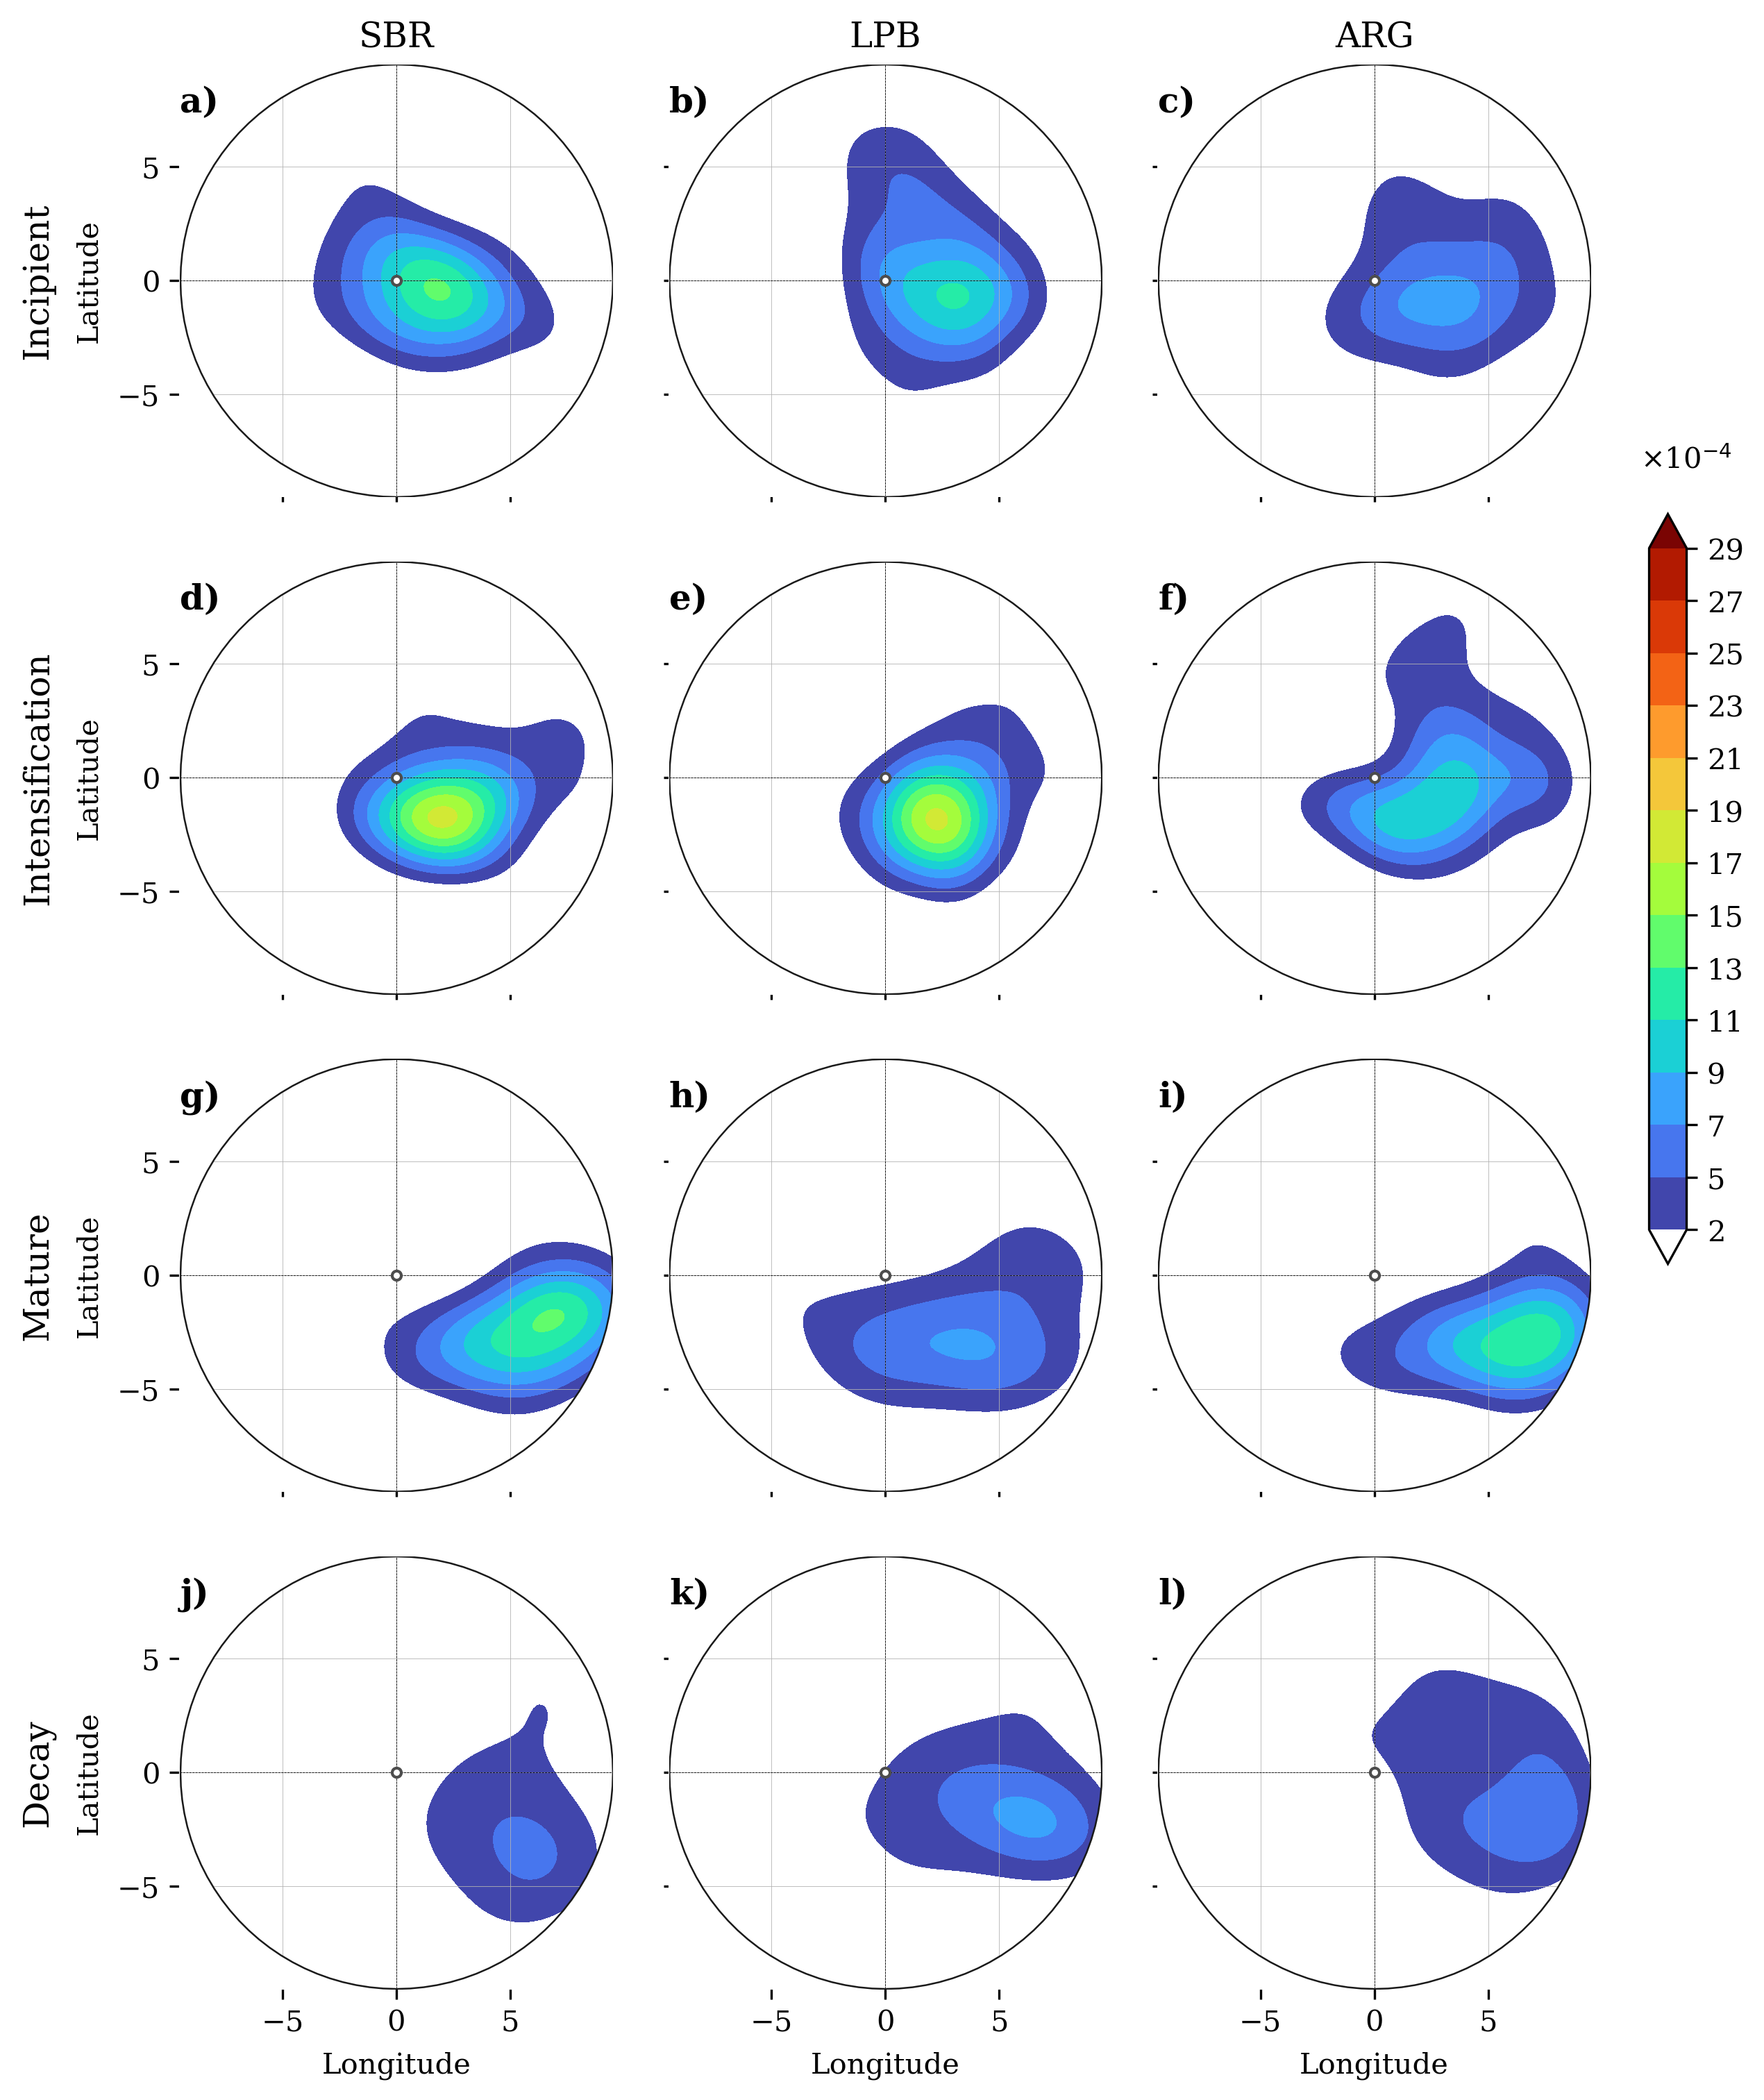
\includegraphics[width=\textwidth]{images/tp/kde_tp_p90_fasesxreg.png}
\caption[Distribución espacial (KDE) de precipitación máxima - Subconjunto p90]{Estimación de densidad espacial bidimensional (KDE) para la ubicación geométrica de los máximos de precipitación total (mm/h) correspondiente al subconjunto de ciclones extremos (percentil 90). El formato de los paneles (a-l), la evolución temporal, la segregación regional y la escala colorimétrica ($10^{-4}$) replican la estructura de la Figura~\ref{fig:kde_tp_global}, permitiendo cuantificar el contraste con la poblacion global.}
\label{fig:kde_tp_p90}
\end{figure}

Al contrastar la distribución base con el estrato de sistemas extremos (p90), la reorganización espacial resulta tan drástica como la observada en el campo de viento, aunque en sentido topológicamente inverso. La Figura~\ref{fig:kde_tp_p90} revela que la arquitectura pluviométrica de los ciclones más intensos no amplifica la concentración oriental de la población general, sino que experimenta una profunda mutación estructural al transitar hacia la madurez (M; paneles g-i). Las densidades máximas de precipitación se alejan del centro de vorticidad $(0,0)$ y se confinan en bandas sumamente estrechas y arqueadas. En las regiones de SBR y LPB, estas zonas de alta probabilidad trazan una geometría fuertemente asimétrica que se concentra en el sector este y sureste, extendiéndose hacia el sur del sistema, dejando el cuadrante central y noroccidental virtualmente desprovistos de máximos de lluvia.

Esta reorganización espacial obedece primariamente al proceso de oclusión rápida propia de ciclones baroclínicos explosivos. Al alcanzar su máxima intensidad, estos vórtices extremos experimentan una violenta intrusión seca (\textit{dry intrusion}): el descenso forzado de aire frío y seco desde la alta troposfera penetra hasta el núcleo del ciclón, erradicando la nubosidad profunda y creando la característica cuña libre de lluvia (\textit{dry slot}) en las inmediaciones del centro \citep{shapiro1999}. Simultáneamente, el flujo ciclónico arrastra el remanente de humedad del Cinturón Transportador Cálido hacia la periferia, confinándolo estrictamente en el frente retrocedido (\textit{bent-back front}). Este proceso genera la clásica banda de precipitación enroscada (\textit{wrap-around precipitation}), una estructura topológicamente cuasi-estacionaria respecto al centro de bajas presiones que explica la geometría arqueada observada en el KDE durante la madurez y el decaimiento \citep{schultz2021antecedents}. La formación de esta banda periférica constituye la firma evolutiva culminante del modelo de Shapiro-Keyser, donde la seclusión cálida aísla térmicamente el núcleo y reorganiza la humedad remanente en una estructura de coma altamente predecible.

Sobre esta geometría impuesta por la dinámica de oclusión, operan secundariamente mecanismos termodinámicos que determinan la intensidad extrema de la precipitación dentro de la banda enroscada. La concentración espacial de los volúmenes pluviométricos máximos responde a procesos de subescala que mantienen tasas de condensación elevadas en la periferia del sistema ocluido. \citet{priestley2022improved} destacan que la intensidad máxima de las precipitaciones está estrictamente condicionada por la fuerza del WCB residual y la presencia de convección profunda embebida a lo largo del frente frío o en el núcleo del frente ocluido. Esta convección embebida, documentada por \citet{oertel2021warm} y \citet{blanchard2021warm}, desencadena corrientes verticales veloces que incrementan drásticamente el contenido local de hidrometeoros mediante la liberación intensa de calor latente. La retroalimentación diabática asociada inyecta masas de aire con baja vorticidad potencial en la tropopausa, alterando los gradientes térmicos e intensificando la circulación local, lo que sostiene rigidamente el patrón pluviométrico periférico frente a la intrusión seca central.

A escala de proceso, las tasas extremas puntuales dentro de esta banda enroscada se generan mediante circulaciones inclinadas de mesoescala (\textit{slantwise circulations}) asociadas a la cabeza de nube del frente ocluido. Como demuestran \citet{clark2005sting}, en eventos desarrollados sobre regiones de alta disponibilidad de humedad superficial como SBR y LPB, estas circulaciones ascendentes convectivas y baroclínicas generan condensación extremadamente rápida. Esta retroalimentación termodinámica local, impulsada por inestabilidades dinámicas en el entorno del frente retrocedido, justifica las densidades espaciales agudas y localizadas que dominan la matriz del percentil p90, distinguiendo estos sistemas de la precipitación estratiforme moderada de la población global.

La consolidación y mantenimiento de esta arquitectura singular dependen contextualmente de los forzantes de superficie del Atlántico subtropical. Los intensos flujos de calor latente y sensible desde el océano hacia la atmósfera, modelados por \citet{gozzo2013air} para ciclones tipo Shapiro-Keyser en esta región, calientan la baja troposfera y sostienen la convección en la vecindad del frente retrocedido. Complementariamente, \citet{andrade2024composite} evidencian que la advección de aire frío y seco sobre aguas oceánicas cálidas genera gradientes verticales de humedad que inducen evaporación masiva, cuya condensación posterior organiza rígidamente el patrón pluviométrico periférico. Estos flujos oceánico-atmosféricos actúan como condicionantes necesarios que permiten alcanzar el estatus de p90, aunque no determinan por sí solos la geometría enroscada, que es inherente a la dinámica de oclusión.

La cuantificación de esta arquitectura espacialmente desacoplada completa la teoría del riesgo compuesto en el Atlántico Sur. De acuerdo con el marco conceptual de \citet{zscheischler2018future}, los peligros meteorológicos extremos surgen de la combinación de múltiples procesos físicos interactuando a diferentes escalas. En las regiones SBR y LPB, los núcleos del percentil p90 representan la superposición espaciotemporal de: (i) la convergencia sinóptica inducida por el ciclón ocluido, (ii) el forzante mesoescala de convección embebida en la banda enroscada, y (iii) la fuente de humedad oceánica que sostiene la condensación. Esta configuración implica que, en ciclones extremos maduros, los forzantes destructivos operan en cuadrantes opuestos: mientras las ráfagas de viento más severas se hiperconcentran en el sector noroeste (asociadas a la cinta transportadora fría), los máximos remanentes de lluvia son empujados hacia el sureste y sur, orbitando el margen exterior de la intrusión seca. Este hallazgo exige una reestructuración de los sistemas de alerta temprana multicomponente, confirmando que el epicentro del peligro hidrológico y el epicentro del peligro eólico en eventos severos no colisionan geográficamente, sino que impactan de manera desfasada y en regiones espaciales mutuamente excluyentes.

% ==============================================================================
% SECCIÓN: PATRONES DOMINANTES DE VARIABILIDAD (EOF) - PRECIPITACIÓN
% ==============================================================================
\section{Organización estructural: Análisis EOF}\label{sec:eof_tp}
\subsection{Fraccionamiento de varianza}\label{subsec:var_exp_tp}
% ==============================================================================

\begin{figure}[htbp]
\centering
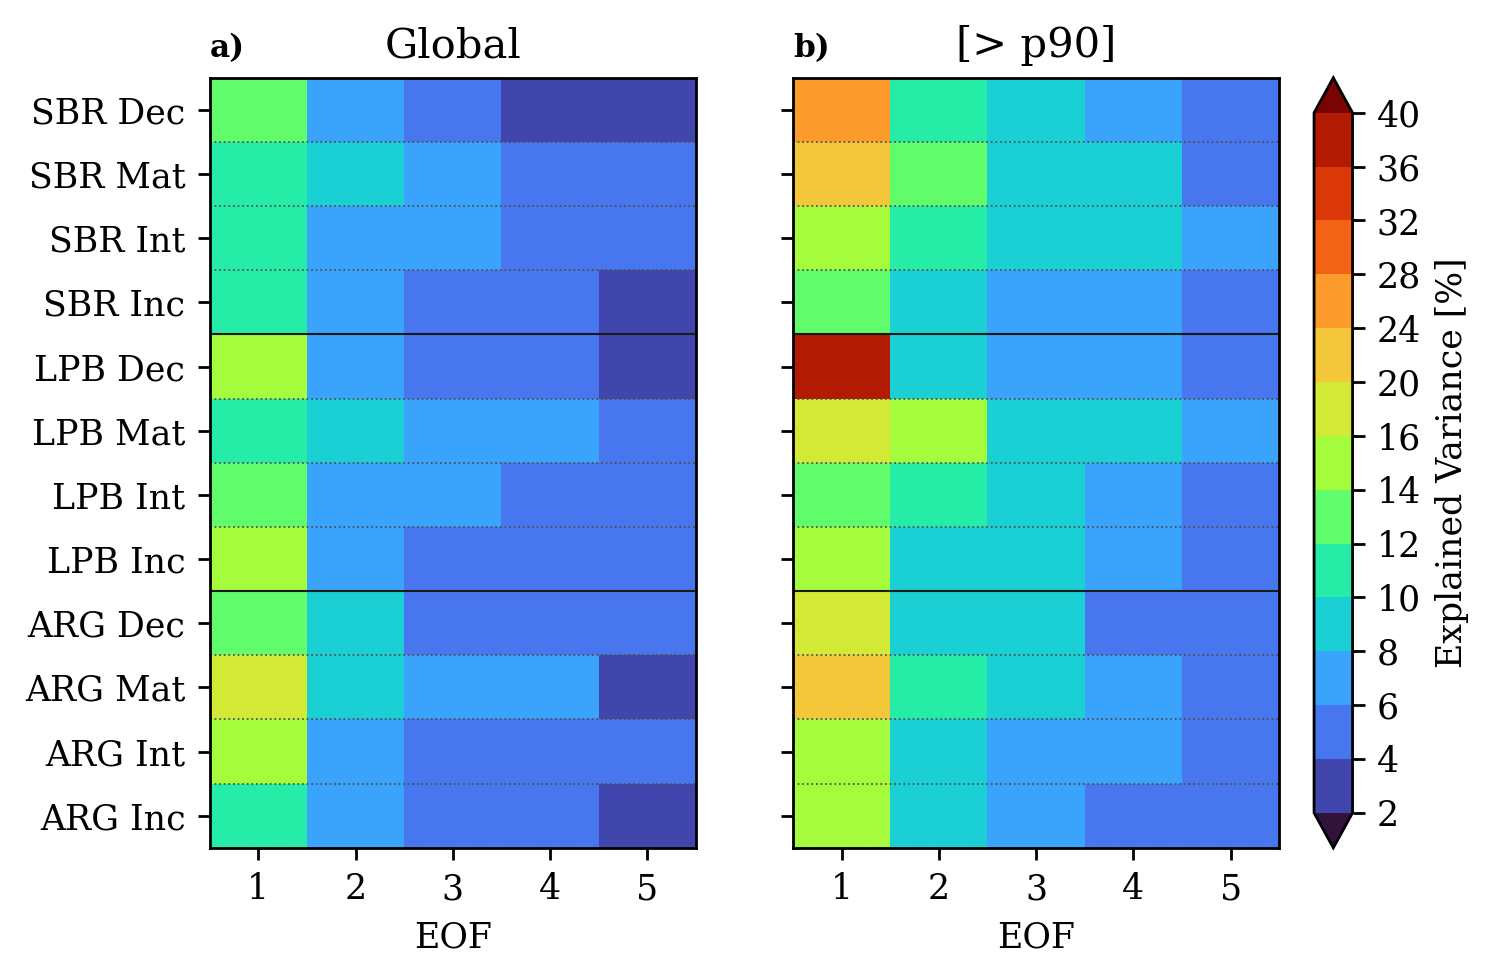
\includegraphics[width=\textwidth]{images/tp/all_expvar_tp_mean2times.png}
\caption[Varianza explicada por los primeros cinco modos (EOF1-EOF5) de precipitación]{Fraccionamiento de la varianza espacial total contenida en los primeros cinco modos dominantes (EOF1 a EOF5) del campo de precipitación total. Se contrasta la distribución de la varianza de la Población Global frente al subconjunto de intensidad (p90) a lo largo del ciclo de vida para cada región de ciclogénesis.}
\label{fig:var_exp_tp}
\end{figure}

La Figura~\ref{fig:var_exp_tp} presenta la distribución porcentual de la varianza espacial explicada por cada uno de los cinco primeros modos empíricos (PC1 a PC5), organizada en una matriz de mapas de calor. Las columnas contrastan la Población Global (panel a) contra los subconjuntos de intensidad extrema (p90, panel b). Las filas corresponden a las doce combinaciones de región de ciclogénesis (SBR, LPB, ARG) y fase evolutiva (incipiente, intensificación, madurez y decaimiento), siguiendo la misma convención matricial empleada en los campos KDE. La escala cromática cuantifica el porcentaje de varianza explicada, donde los tonos azules y verdes indican baja concentración de varianza (modos dispersos) y los tonos amarillos y rojos revelan alta concentración en el modo principal.

Visualmente, el contraste entre paneles es marcado: mientras que la Población Global (a) y los estratos moderados (c) y débiles (d) exhiben predominantemente tonos fríos distribuidos uniformemente entre los cinco modos, el panel de sistemas extremos (b) muestra tonos cálidos concentrados en la primera columna (PC1) durante las fases finales del ciclo de vida. Específicamente, en el decaimiento de LPB y SBR, el PC1 alcanza valores superiores al 35\% y 25\% respectivamente, mientras que en la Población Global estos mismos casos apenas superan el 10\%. Esta transición cromática de frío a cálido en el estrato p90 constituye la evidencia visual del colapso dimensional que caracteriza a los ciclones extremos en su fase final.

El análisis de esta distribución revela un patrón marcadamente distinto al observado en las variables cinemáticas. Mientras que en el viento el modo dominante concentra la mayor parte de la variabilidad, en la precipitación la varianza se distribuye de manera aplanada entre múltiples modos durante las fases incipiente, intensificación y madurez de la Población Global %, así como en los estratos de baja y moderada intensidad (p10 y p50). 
Este comportamiento disperso contrasta abruptamente con el salto observado en los sistemas extremos (p90) al ingresar en la fase de decaimiento, donde el EOF1 alcanza el 36,5\% en LPB y el 26,2\% en SBR, superando con creces los valores típicos de la climatología general (entre 11\% y 16\%).

El aplanamiento generalizado del espectro de varianza en la precipitación responde a la naturaleza espacialmente discontinua de este campo. A diferencia de las variables de masa o cinemáticas, que obedecen a gradientes continuos de gran escala, la lluvia está gobernada por frentes activos de escala muy reducida, núcleos de convección embebida y tasas asimétricas de liberación de calor latente \citep{oertel2021warm}. Esta fragmentación espacial implica que ningún único patrón espacial puede capturar la diversidad de configuraciones pluviométricas presentes en la muestra. De acuerdo con los criterios de interpretación EOF establecidos por \citet{hannachi2007empirical}, la distribución de la varianza entre múltiples modos indica que el campo pluviométrico es inherentemente heterogéneo, exigiendo la retención de varios modos ortogonales para reconstruir adecuadamente la variabilidad observada. En este sentido, \citet{graf2017objective} revelan que la ciclogénesis no opera en categorías discretas, sino en un continuo físico donde los procesos húmedos y la producción diabática de vorticidad potencial constituyen dimensiones de variabilidad cuasi-independientes, lo que explica la dispersión de la energía entre EOF2 y EOF5 durante las fases iniciales en todas las regiones.

El comportamiento distintivo de los sistemas extremos (p90) durante el decaimiento, donde el EOF1 concentra hasta el 36,5\% de la varianza en LPB, obedece a la consolidación de la banda enroscada (*wrap-around precipitation*) como estructura dominante. Cuando los ciclones severos alcanzan la fase final de su ciclo de vida, la intrusión seca y el frente retrocedido organizan la precipitación remanente en una geometría espacial rígidamente coherente y cuasi-estacionaria respecto al centro del vórtice. Esta organización estructural reduce drásticamente la heterogeneidad espacial que caracteriza a los sistemas moderados, permitiendo que un único modo espacial capture la configuración pluviométrica dominante. Como señalan \citet{hannachi2023eof}, el análisis EOF permite examinar sistemas complejos mediante la descomposición de su matriz de covarianza espacial, y en este caso particular, la consolidación de la banda periférica durante el decaimiento genera una reducción dimensional efectiva donde el primer modo retiene la mayor fracción posible de la varianza total del campo.

Las diferencias regionales en el fraccionamiento de varianza reflejan la influencia de los forzantes orográficos y térmicos estacionarios del Hemisferio Sur. De acuerdo con \citet{inatsu2004zonal}, la génesis y el desarrollo del tren de ondas baroclínicas presentan una marcada asimetría zonal, forzada por la interrupción del flujo que supone la cordillera de los Andes y por los contrastes térmicos mar-tierra. Esta modulación dinámica a gran escala fija zonas preferenciales de ciclogénesis y áreas recurrentes de frontogénesis, lo que explica que regiones como ARG o el oeste de LPB presenten valores ligeramente superiores de varianza explicada por el EOF1 durante las fases iniciales respecto a SBR, donde la influencia oceánica y la convección tropical introducen mayor variabilidad estructural.

Desde una perspectiva metodológica, la técnica EOF resulta apropiada para este análisis porque transforma el conjunto de datos atmosféricos interdependientes en nuevas variables espacialmente ortogonales diseñadas para capturar la máxima fracción posible de la varianza total en cada modo sucesivo \citep{wilks2019statistical_ch13}. Aunque en la Población Global esta varianza queda distribuida entre varios modos, la descomposición permite aislar la respuesta dominante del sistema respecto a las anomalías estructurales de menor escala. 

Esta confirmación cuantitativa resulta metodológicamente trascendental. Demuestra que el impacto pluviométrico en sistemas ordinarios es difuso, justificando la necesidad de retener múltiples modos espaciales para su descripción completa. Sin embargo, también prueba contundentemente que los eventos extremos (p90) poseen la capacidad singular de organizar las precipitaciones remanentes en geometrías rígidamente coherentes al final de su ciclo de vida, fenómeno que no tiene equivalente en los campos cinemáticos y que constituye una firma diagnóstica distintiva de los sistemas severos del Atlántico Sur.
%%
%%%%
%%%%%%
%%%%
%%
% ==============================================================================
\subsection{Patrones espaciales dominantes (EOF1)}\label{subsec:eof1_tp}
% ==============================================================================

% 
\subsubsection{Población Global}\label{subsubsec:eof1_tp_global}

\begin{figure}[htbp]
\centering
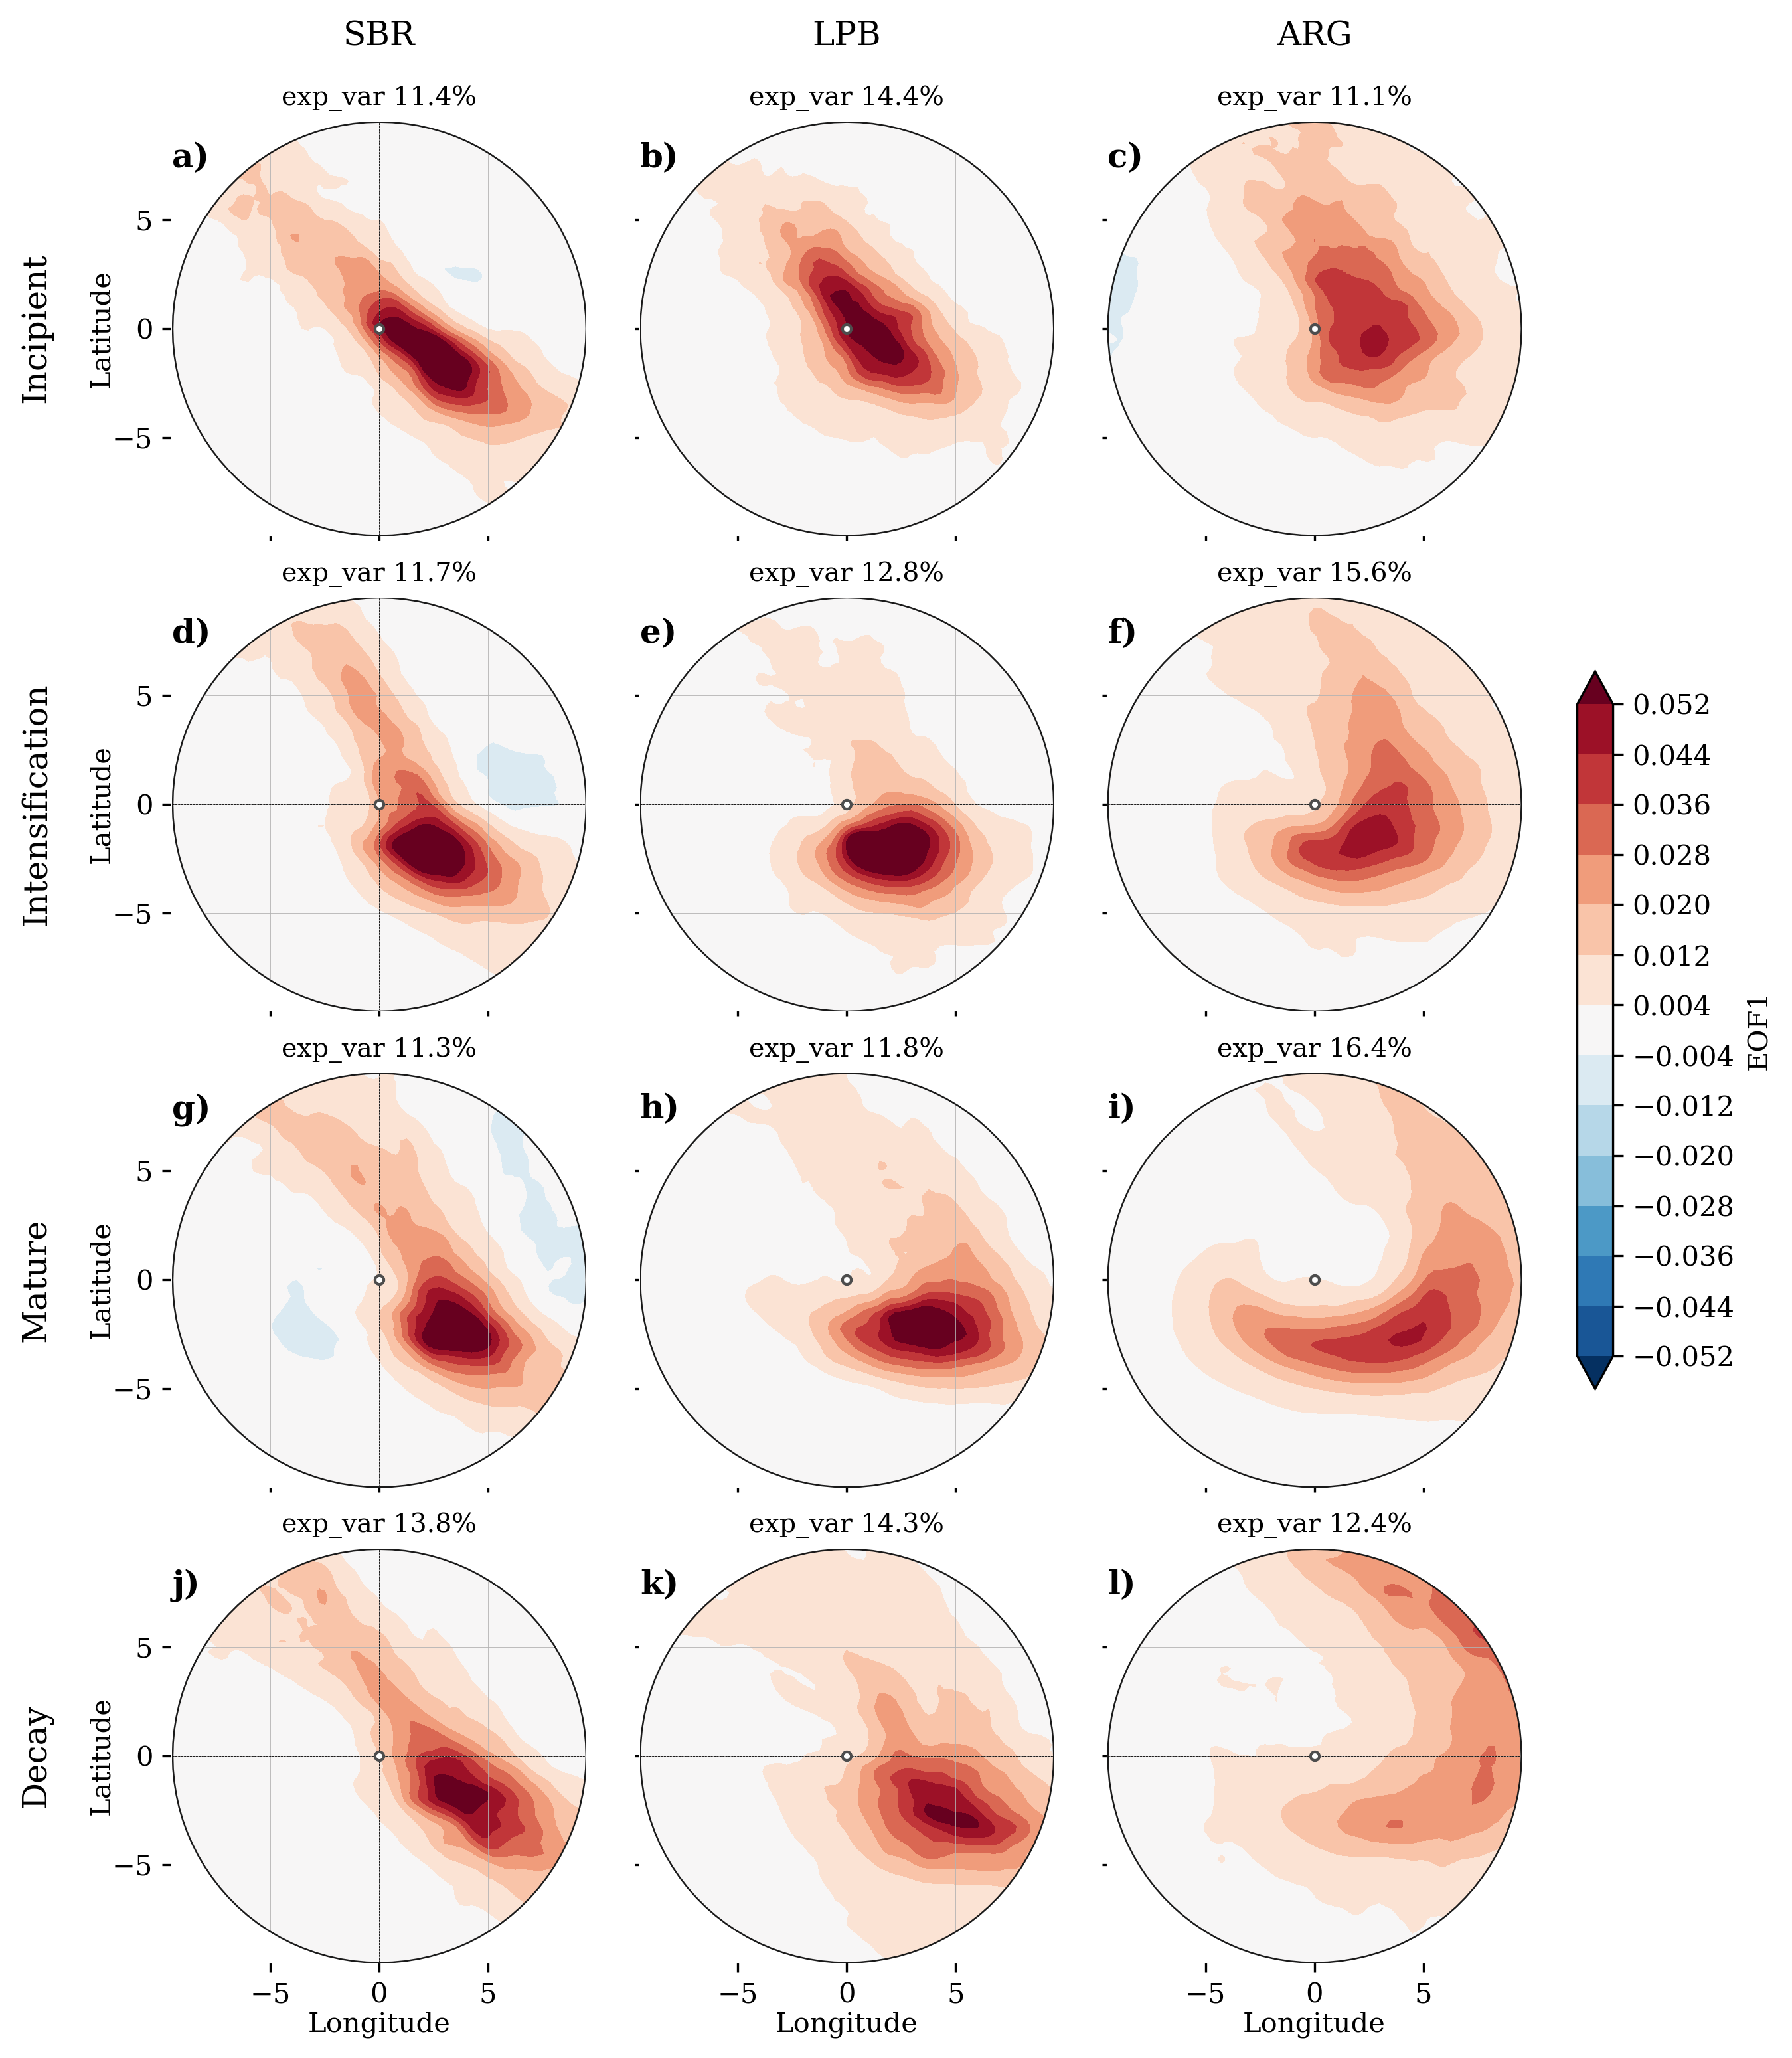
\includegraphics[width=\textwidth]{images/tp/pca1_tp_global_fasesxreg.png}
\caption[EOF1 de precipitación total - Población Global]{Primer modo espacial (EOF1) de la precipitación total (mm/h) para la Población Global de referencia. La disposición matricial organiza la evolución por regiones de ciclogénesis en columnas (SBR, LPB y ARG) y las fases de desarrollo evolutivo en filas (Incipiente, Intensificación, Madurez y Decaimiento). Sobre cada panel se indica el porcentaje de la varianza espacial total explicada (\textit{exp\_var}) por esta componente principal. La escala cromática divergente cuantifica las anomalías estructurales relativas al centro del vórtice.}
\label{fig:eof1_tp_global}
\end{figure}

La Figura~\ref{fig:eof1_tp_global} presenta los patrones espaciales correspondientes al primer modo empírico (EOF1) de la precipitación total, siguiendo la misma disposición matricial de 4 filas (fases) por 3 columnas (regiones) empleada en los campos KDE previos. Cada panel muestra un dominio circular lagrangiano de 20 grados centrado en el vórtice (punto blanco), con contornos de colores que representan las anomalías estructurales de precipitación respecto a la media. A diferencia del patrón dipolar simétrico observado en el EOF1 del viento a 10 metros (Sección~\ref{subsubsec:eof1_wind10_global}), donde las anomalías positivas y negativas se distribuyen en sectores opuestos bien definidos, aquí el modo dominante exhibe una organización marcadamente asimétrica: las anomalías positivas (tonos rojizos y marrones) se concentran preferentemente en el sector oriental y suroriental del dominio, mientras que los valores negativos (tonos azules) aparecen de manera fragmentada y de menor magnitud. Los porcentajes de varianza explicada anotados en cada panel oscilan entre el 11,1\% y el 16,4\%, confirmando visualmente la baja dominancia del primer modo respecto a la variables cinemáticas. Esta distribución irregular, con contornos difusos y múltiples focos de máximos en lugar de un único núcleo simétrico, refleja la naturaleza inherentemente discontinua del campo pluviométrico.

El patrón espacial observado obedece primariamente a la organización dinámica del Cinturón Transportador Cálido (WCB). Según el modelo conceptual de \citet{browning1986conceptual}, el ascenso inclinado del WCB por delante del frente frío y por encima del frente cálido organiza inherentemente la precipitación en el flanco cálido del ciclón. En el contexto del Atlántico Sudoccidental, este flujo termodinámico obligatorio configura el esqueleto espacial base que se observa en las tres regiones: una banda de anomalías positivas orientada de noroeste a sureste, coincidente con la trayectoria del aire ascendente en el sector cálido del sistema. La variabilidad capturada por el EOF1 representa, por tanto, las fluctuaciones en la intensidad y posición de esta corriente ascendente a medida que el ciclón evoluciona.

Sobre este esqueleto dinámico del WCB, operan moduladores regionales que explican las diferencias en la intensidad del patrón entre SBR, LPB y ARG. La disponibilidad de humedad para alimentar el WCB está condicionada por el transporte remoto de vapor de agua desde el Atlántico tropical hacia las zonas baroclínicas activas. De acuerdo con \citet{gozzo2017climatology}, la ciclogénesis en el Atlántico Sudoccidental está profundamente supeditada a este aporte de humedad remota, sumada a los flujos locales de calor latente por evaporación sobre la superficie oceánica. Esta configuración explica por qué el patrón del EOF1 en SBR y LPB presenta anomalías más intensas y concentradas cerca de la costa occidental, donde la convergencia de humedad es máxima, mientras que en ARG el patrón es más difuso y desplazado hacia el noreste.
%
% El mecanismo físico específico que canaliza esta humedad hacia el sector cálido del ciclón reside en los patrones de circulación en niveles bajos de la troposfera. Como documentan \citet{rocha2016estudo}, la convergencia del viento en 850 hPa es decisiva para estimular la ciclogénesis, evidenciando el rol del transporte de humedad desde regiones continentales, en SBR y LPB estas áreas de carga positiva en el EOF1 coinciden en los primeros tiempos de la formacion del ciclon, evidenciando el rol del aporte de vapor de agua marino. Este ingreso constante desde el océano abierto hacia la franja continental actúa como el motor de la precipitación, validando que la variabilidad dominante capturada por el análisis EOF responde a fluctuaciones en la eficiencia de este transporte de humedad costero.
%
El mecanismo físico que explicaría la señal positiva de la EOF1 reside en los patrones de circulación de los bajos niveles de la troposfera. Como documentan \citet{rocha2016estudo}, la convergencia en 850 hPa estimula la ciclogénesis en el Atlántico Sur. Esta convergencia facilita un transporte constante de humedad desde regiones como la Amazonía, el cual se concentra en la zona de formación del sistema en SBR y LPB. La coincidencia espacial entre la variabilidad de la EOF1 y las áreas de convergencia identificadas por el autor sugiere una respuesta a la eficiencia de este transporte de humedad y a la liberación de calor latente aporta para la precipitación en este sector del ciclon.

% La naturaleza de contornos observada en el EOF1, particularmente durante las fases incipientes, responde a la intermitencia inherente de los procesos convectivos. Como señalan \citet{naud2020evaluation}, la convección en el sector cálido se organiza en regiones de fuerte ascenso y altos niveles de humedad, En esta región, la intensidad de la precipitación está estrechamente vinculada a la fuerza del ascenso dinámico, lo que genera núcleos de precipitación que contrastan con la naturaleza intermitente de otras áreas del ciclón. Por otro lado, \citet{hannachi2007empirical} explica que la baja varianza del primer modo se debe a los campos altamente variables. En el caso de la precipitacion se espera esta limitacion de la varianza explicada debido a que la EOF a menudo le es dificil capturar de procesos físicos localizados e intermitentes.
La distribución espacial capturada por el EOF1, refleja la naturaleza intermitente y localizada inherente a los procesos convectivos de precipitación. Como señalan \citet{naud2020evaluation}, la convección en el sector cálido se organiza en regiones de ascenso dinámico y de convergencia de humedad. En esta región, la intensidad de la precipitación está estrechamente vinculada a la fuerza de dicho ascenso, lo que genera núcleos de precipitación que contrastan marcadamente con las áreas libres de precipitación o de llovizna dispersa en el resto del ciclón. Por otro lado, desde una perspectiva estadística, \citet{hannachi2007empirical} explican que la baja varianza explicada por el primer modo se debe, precisamente, al carácter altamente variable del campo analizado. En el caso específico de la precipitación, esta limitación en la varianza es esperable, ya que el análisis EOF a menudo tiene dificultades para capturar eficientemente procesos físicos no lineales que son, por naturaleza, localizados e intermitentes
%
La extracción de este modo univariado para la climatología general confirma que, en un escenario promedio, las fluctuaciones pluviométricas carecen de una simetría centralizada duradera y se rigen por la variabilidad transitoria del sector frontal oriental. Establecer esta línea base dispersa permite dimensionar objetivamente la magnitud de la transformación estructural que experimentan los eventos severos (p90), los cuales, al alcanzar la madurez y ocluirse, abandonan este comportamiento transitorio para confinar la precipitación en geometrías rígidamente estructuradas, como se examina a continuación.

% 
\subsubsection{Subconjunto p90}\label{subsubsec:eof1_tp_p90}
% 
\begin{figure}[htbp]
\centering
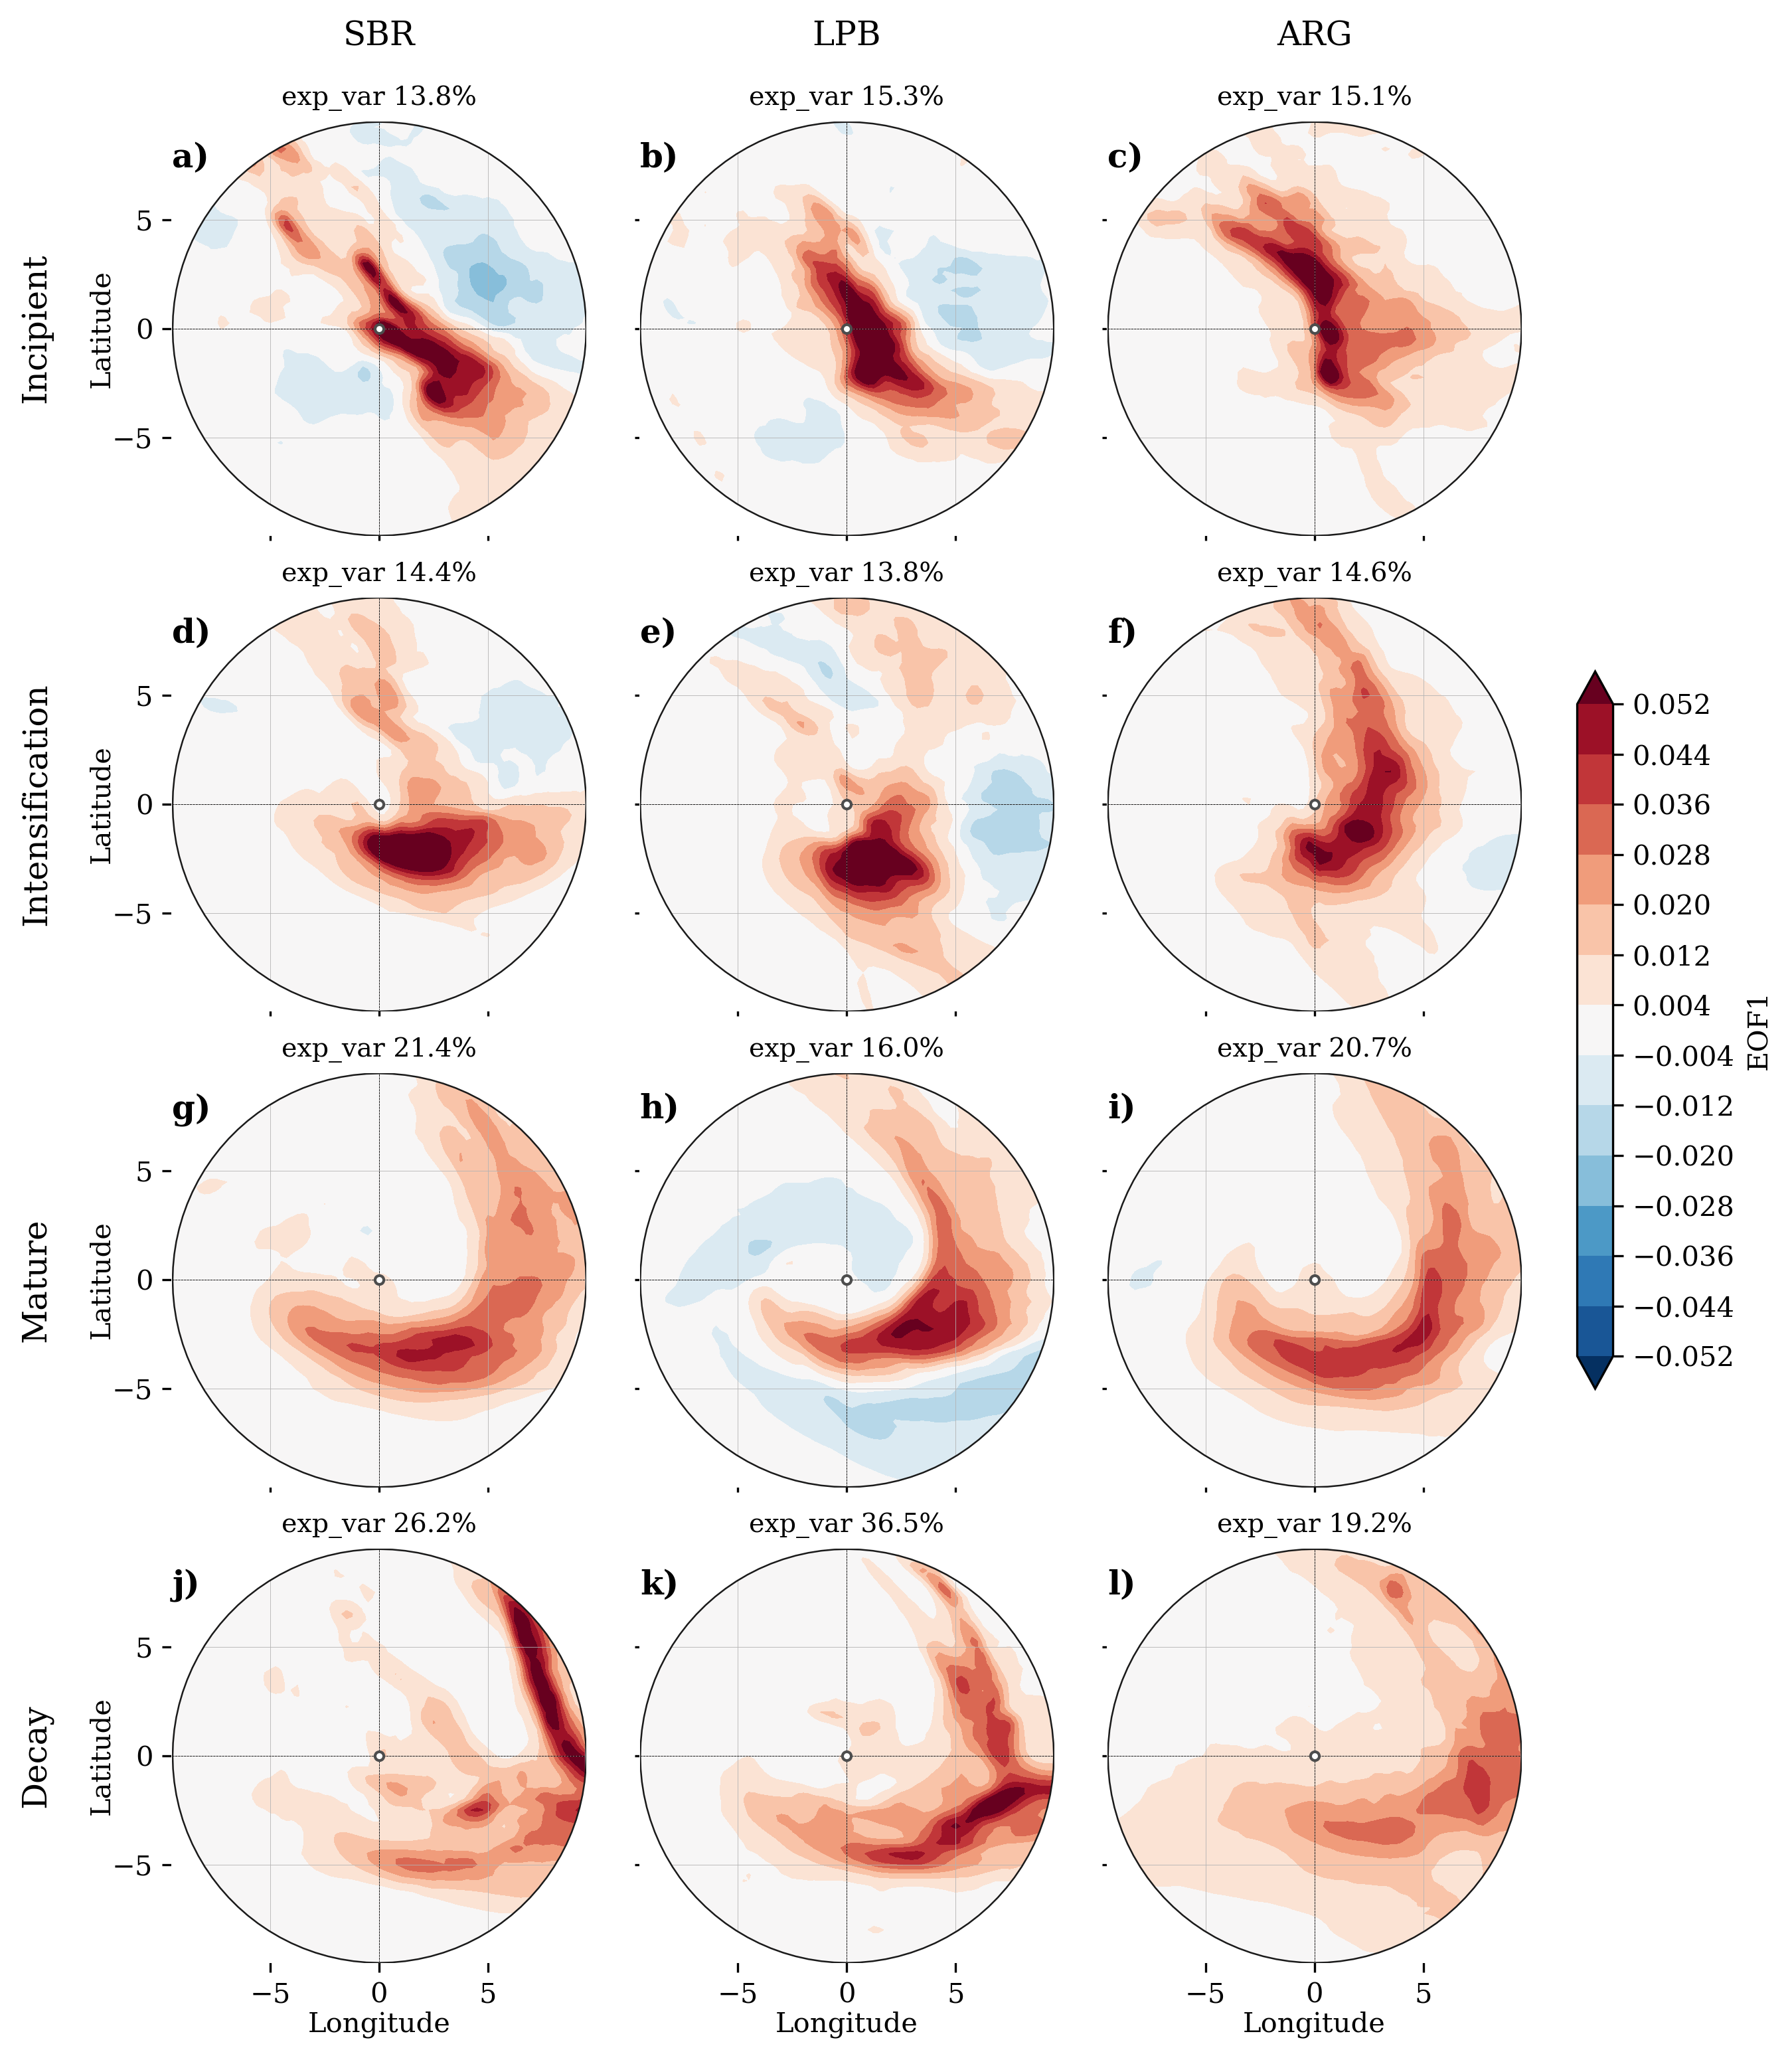
\includegraphics[width=\textwidth]{images/tp/pca1_tp_p90_fasesxreg.png}
\caption[EOF1 de precipitación total - Subconjunto p90]{Primer modo espacial (EOF1) de la precipitación total (mm/h) para el estrato de ciclones extremos (percentil 90). El formato de los paneles (a-l), la nomenclatura de varianza explicada y el dominio espacial mantienen una correspondencia estricta con la Figura~\ref{fig:eof1_tp_global}, permitiendo cuantificar la profunda transformación estructural que experimentan los sistemas severos, especialmente durante su oclusión final.}
\label{fig:eof1_tp_p90}
\end{figure}

La Figura~\ref{fig:eof1_tp_p90} presenta los patrones espaciales del primer modo empírico para el estrato de ciclones extremos, manteniendo la disposición matricial de doce paneles utilizada en la población global. El contraste visual con la Figura~\ref{fig:eof1_tp_global} es inmediato: mientras que en la población general los valores de varianza explicada oscilaban entre 11\% y 16\%, aquí se observa un salto cuantitativo en las fases finales, alcanzando el 21,4\% en SBR Madurez, el 36,5\% en LPB Decaimiento y el 26,2\% en SBR Decaimiento. Morfológicamente, durante las fases de incipiencia e intensificación (paneles a-f), el EOF1 mantiene patrones irregulares anclados al sector oriental, similares aunque más intensos que los de la población global. Sin embargo, al transitar hacia la madurez y el decaimiento (paneles g-l), se produce una reorganización estructural drástica: el patrón caótico es reemplazado por una firma geométrica nítida y coherente. En SBR (panel j), esta firma consiste en una banda anómala arqueada que se concentra en el sector sureste y se extiende hacia el sur del vórtice; en LPB (panel k), la estructura positiva es más amplia y envuelve el sistema desde el noreste hasta el sureste, con una marcada anomalía negativa en el centro-sur. En ambas regiones, el cuadrante central y noroccidental queda virtualmente libre de anomalías positivas. Esta configuración asimétrica, especialmente evidente durante el decaimiento, contrasta marcadamente con la dispersión difusa observada en los sistemas moderados.

La emergencia de esta estructura espacialmente coherente obedece primariamente al proceso de oclusión severa propia del modelo de Shapiro-Keyser. La fuerte deformación cinemática del vórtice extremo fuerza una intrusión seca profunda desde la alta troposfera que aniquila la convección en el centro geométrico del sistema, creando la característica cuña libre de precipitación. Simultáneamente, el remanente de humedad del Cinturón Transportador Cálido es arrastrado por la intensa circulación ciclónica hacia la periferia, quedando confinado estríctamente en el frente retrocedido \citep{shapiro1990life, schultz2021antecedents}. Esta reorganización genera la banda de precipitación enroscada (*wrap-around precipitation*), una estructura topológicamente cuasi-estacionaria respecto al centro de bajas presiones que explica la geometría arqueada observada en el EOF1 durante las fases finales. Dado que esta banda concentra tasas de precipitación muy superiores a su entorno seco y mantiene una posición relativamente estable respecto al vórtice, el análisis EOF la identifica como la fuente dominante de varianza espacial, justificando el salto abrupto en el porcentaje de energía capturada por el primer modo.

La localización específica y la intensidad de esta banda enroscada dependen secundariamente de las condiciones termodinámicas de la superficie oceánica subyacente. La disponibilidad de humedad forzada por la Temperatura Superficial del Mar y la presencia de núcleos de fuerte ascenso sinóptico modulan la capacidad del sistema para sostener la condensación extrema en la periferia del ciclón ocluido. Como demuestran \citet{Laureanti2024relation} al examinar eventos severos sobre el este y centro de Brasil mediante análisis EOF, los extremos pluviométricos no son fenómenos aislados, sino que están estrictamente ligados a los flujos locales de calor latente desde el océano hacia la atmósfera. Estos flujos calientan la baja troposfera y retroalimentan las corrientes verticales, anclando geográficamente las áreas de máxima varianza y permitiendo que la banda enroscada alcance las tasas de precipitación extremas observadas en el estrato p90, particularmente sobre SBR y la cuenca atlántica adyacente donde el contraste térmico oceánico es más pronunciado.

El mantenimiento de esta arquitectura asimétrica durante el decaimiento responde adicionalmente a procesos de retroalimentación diabática internos. La intensa liberación de calor latente dentro de la banda de precipitación periférica fomenta el aislamiento térmico del núcleo ciclónico. De acuerdo con \citet{reboita2022from}, este calentamiento diabático reduce el cizallamiento vertical del viento y facilita el alineamiento entre los sistemas de niveles bajos y altos, consolidando la seclusión cálida y desacoplando la dinámica pluviométrica de las fluctuaciones lineales del gradiente sinóptico de fondo. Este proceso asegura que la banda enroscada no sea un fenómeno transitorio, sino una estructura robusta que persiste mientras el ciclón se disipa.

Estas transformaciones estructurales pueden situarse dentro del marco conceptual del ciclo de vida ciclónico. Tal como sugieren \citet{hart2003cyclone}, el desarrollo de un ciclón puede evaluarse mediante transiciones de fase que parametrizan la asimetría del espesor relativo y la estructura térmica del núcleo (frío vs. cálido). En el contexto de nuestras regiones de estudio, el paso hacia la madurez y decaimiento en sistemas extremos implica necesariamente el desarrollo de seclusiones cálidas que dictan la ubicación de los forzantes frontogénicos. Sin embargo, es preciso distinguir que este marco describe el contexto evolutivo general, mientras que la forma específica de la banda enroscada observada en el EOF1 deriva directamente de los procesos de oclusión y los forzantes oceánicos descritos precedentemente.

La extracción de esta firma estructural asimétrica y rígida constituye el cierre analítico de las variables individuales. Al contrastar estos patrones con los campos de viento equivalentes (Secciones~\ref{subsubsec:eof1_wind10_p90}), se evidencia geométricamente el desacople espacial de las amenazas: mientras que la variabilidad de las ráfagas destructivas se compacta en el cuadrante noroeste (gobernada por la cinta transportadora fría), la lluvia remanente se organiza en una herradura sólida en los cuadrantes sureste y sur. Este hallazgo valida la necesidad de evaluar los ciclones oceánicos extremos como fenómenos de riesgo compuesto desfasado, donde el epicentro del peligro hidrológico y el epicentro del peligro eólico operan en regiones espaciales mutuamente excluyentes, y provee el respaldo teórico para avanzar hacia el análisis acoplado de ambas variables en el capítulo siguiente.

%%
%%%%
%%%%%%
%%%%
%%

% ==============================================================================
\subsection{Significancia estadística}\label{subsec:significancia_tp}
% ==============================================================================

Para discriminar entre señales físicas robustas y fluctuaciones propias del remuestreo, se evaluó la significancia estadística de los autovectores espaciales mediante el método Bootstrap-$t$ (Sección~\ref{subsec:bootstrap_significancia}). La Figura~\ref{fig:xeof_madurez_global_tp} documenta los tres primeros modos (EOF1--EOF3) y sus respectivas series temporales (PC1--PC3) para la Población Global en fase de madurez, mientras que la Figura~\ref{fig:xeof_madurez_p90_tp} presenta el análisis equivalente para el subconjunto extremo (p90). El achurado delimita las áreas donde las cargas espaciales resultaron estadísticamente significativas al 95\% de confianza.

\begin{figure}[htbp]
\centering
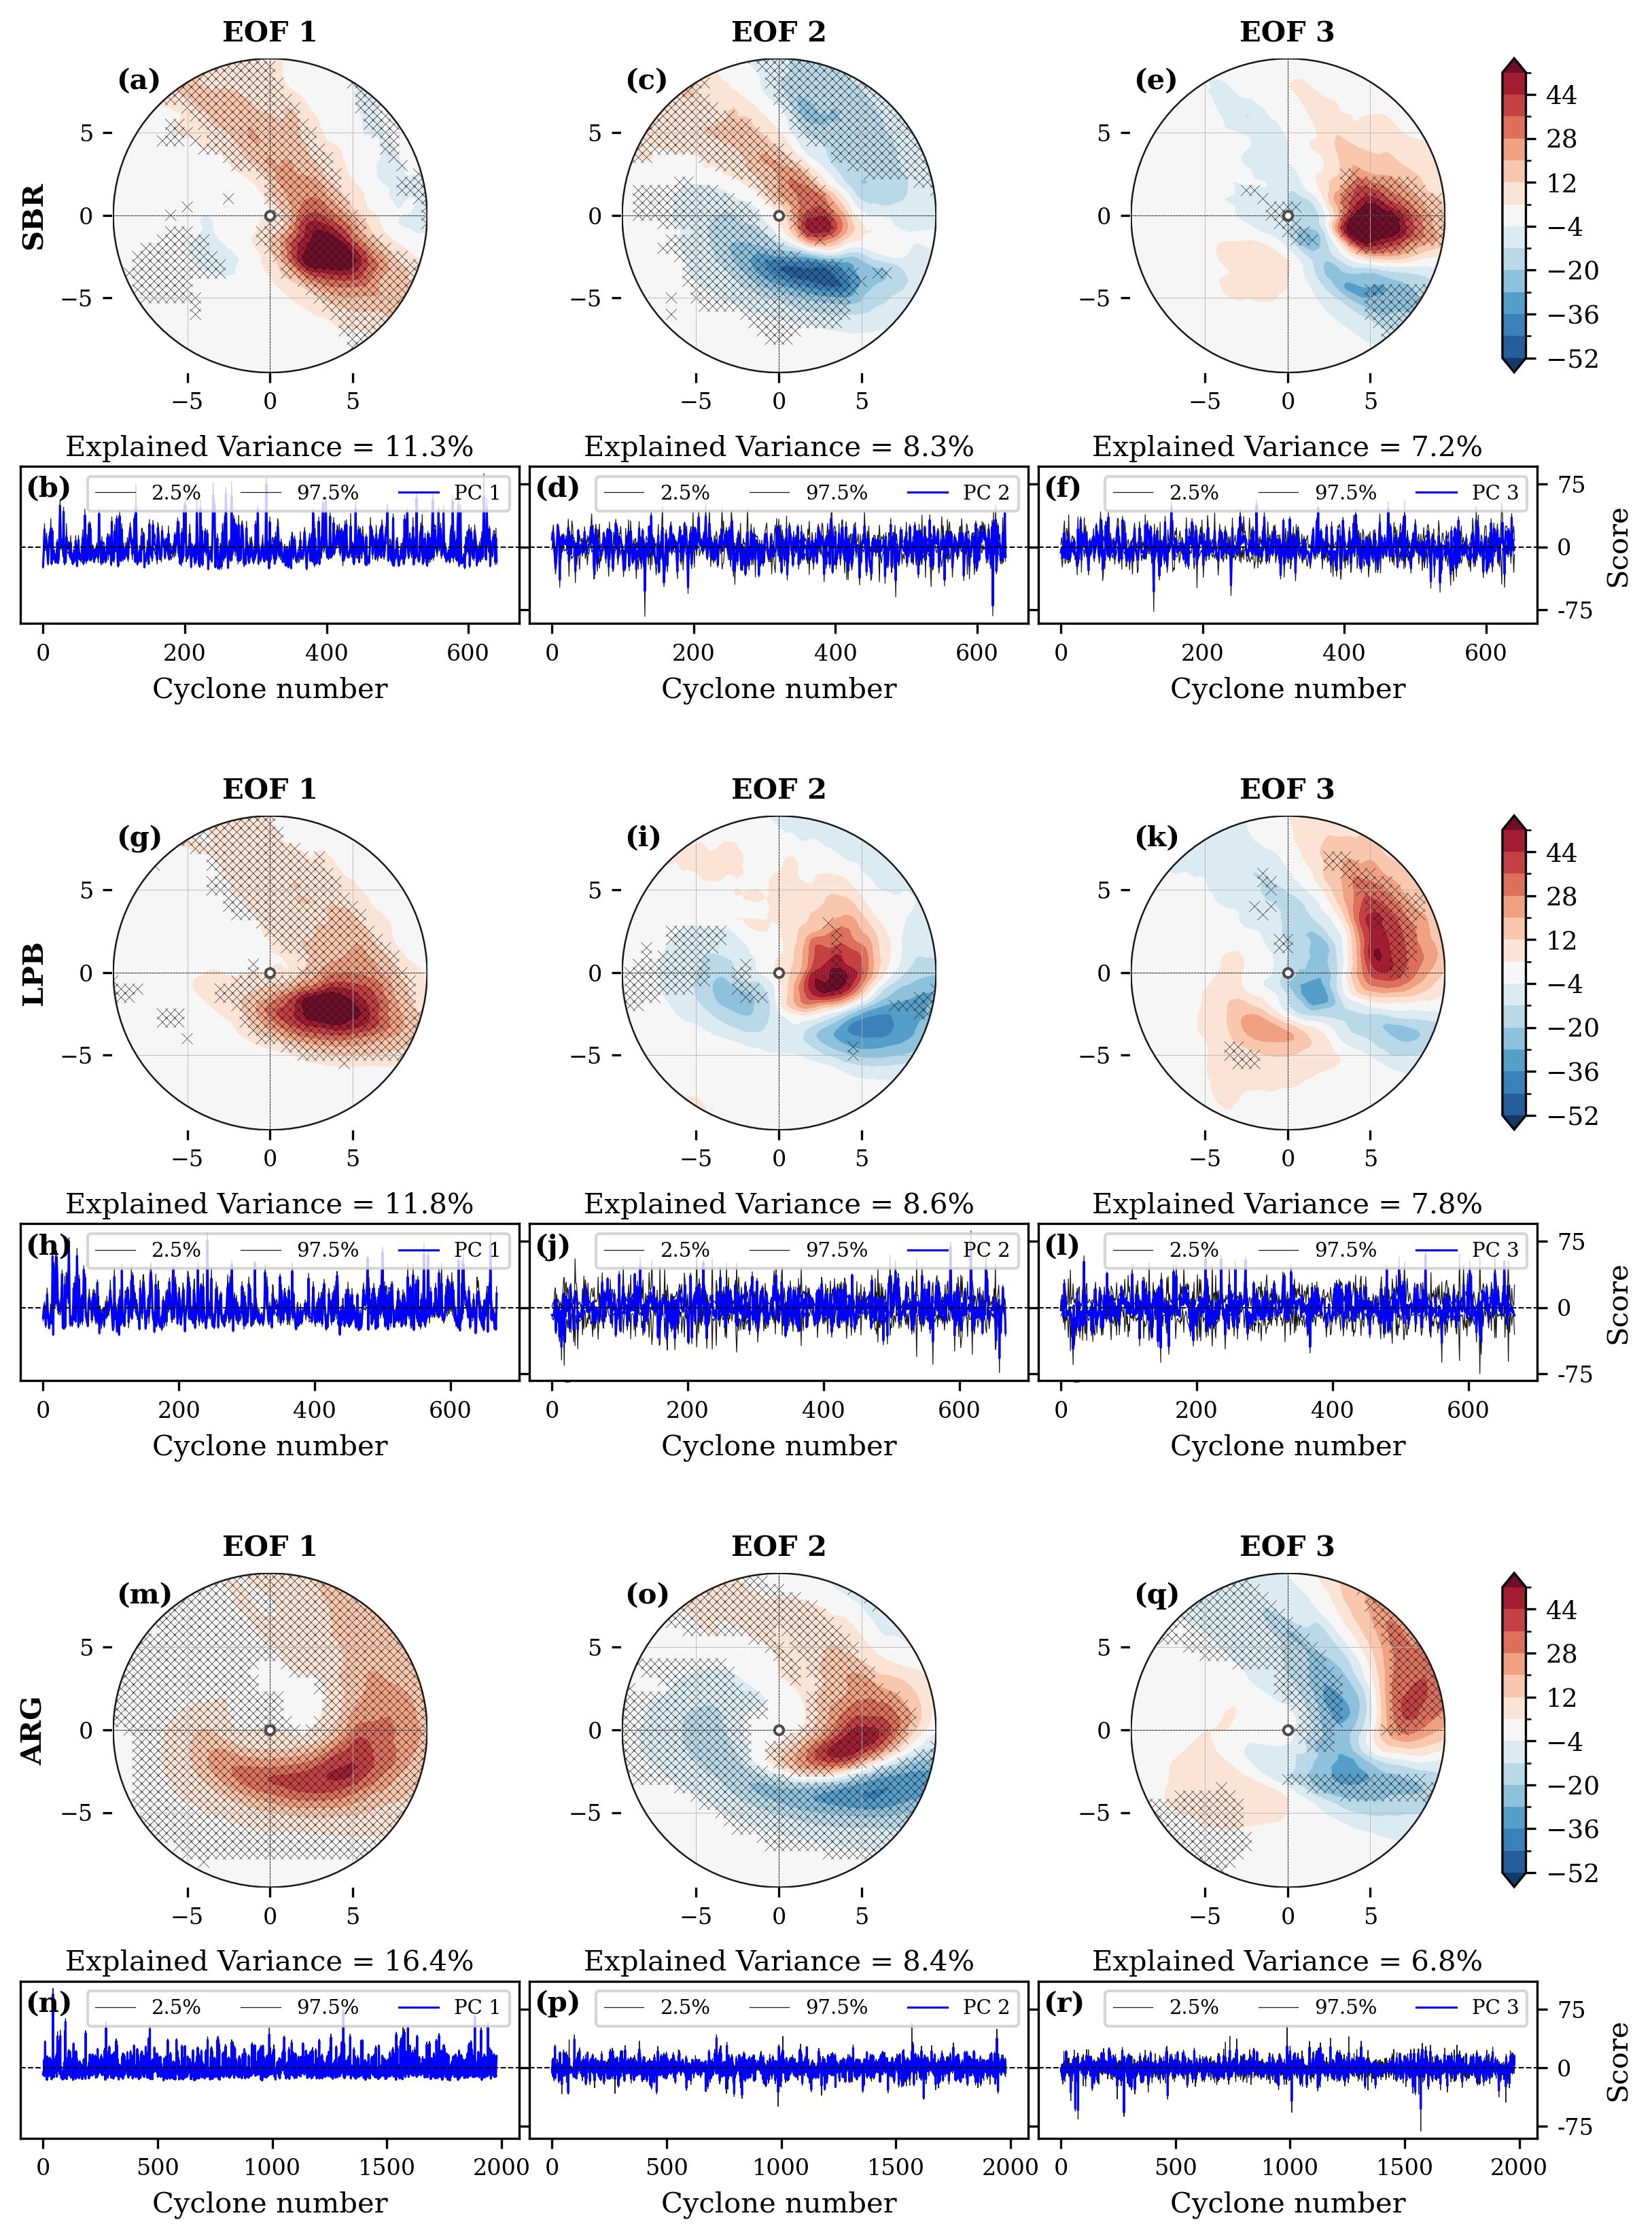
\includegraphics[width=\textwidth]{images/tp/xeof_global_tp_mature.png}
\caption[Significancia espacial de los EOFs en fase de madurez - Población Global (tp)]{Descomposición EOF de la precipitación total para la Población Global en fase de madurez. Paneles (a, c, e): mapas de los tres primeros modos espaciales (EOF1--EOF3) con achurado indicando significancia estadística al 95\% (test Bootstrap-$t$). Paneles (b, d, f): series temporales correspondientes de las Componentes Principales (PC1--PC3). La línea gris delimita los percentiles 2.5 y 97.5 de la distribución bootstrap.}
\label{fig:xeof_madurez_global_tp}
\end{figure}

\begin{figure}[htbp]
\centering
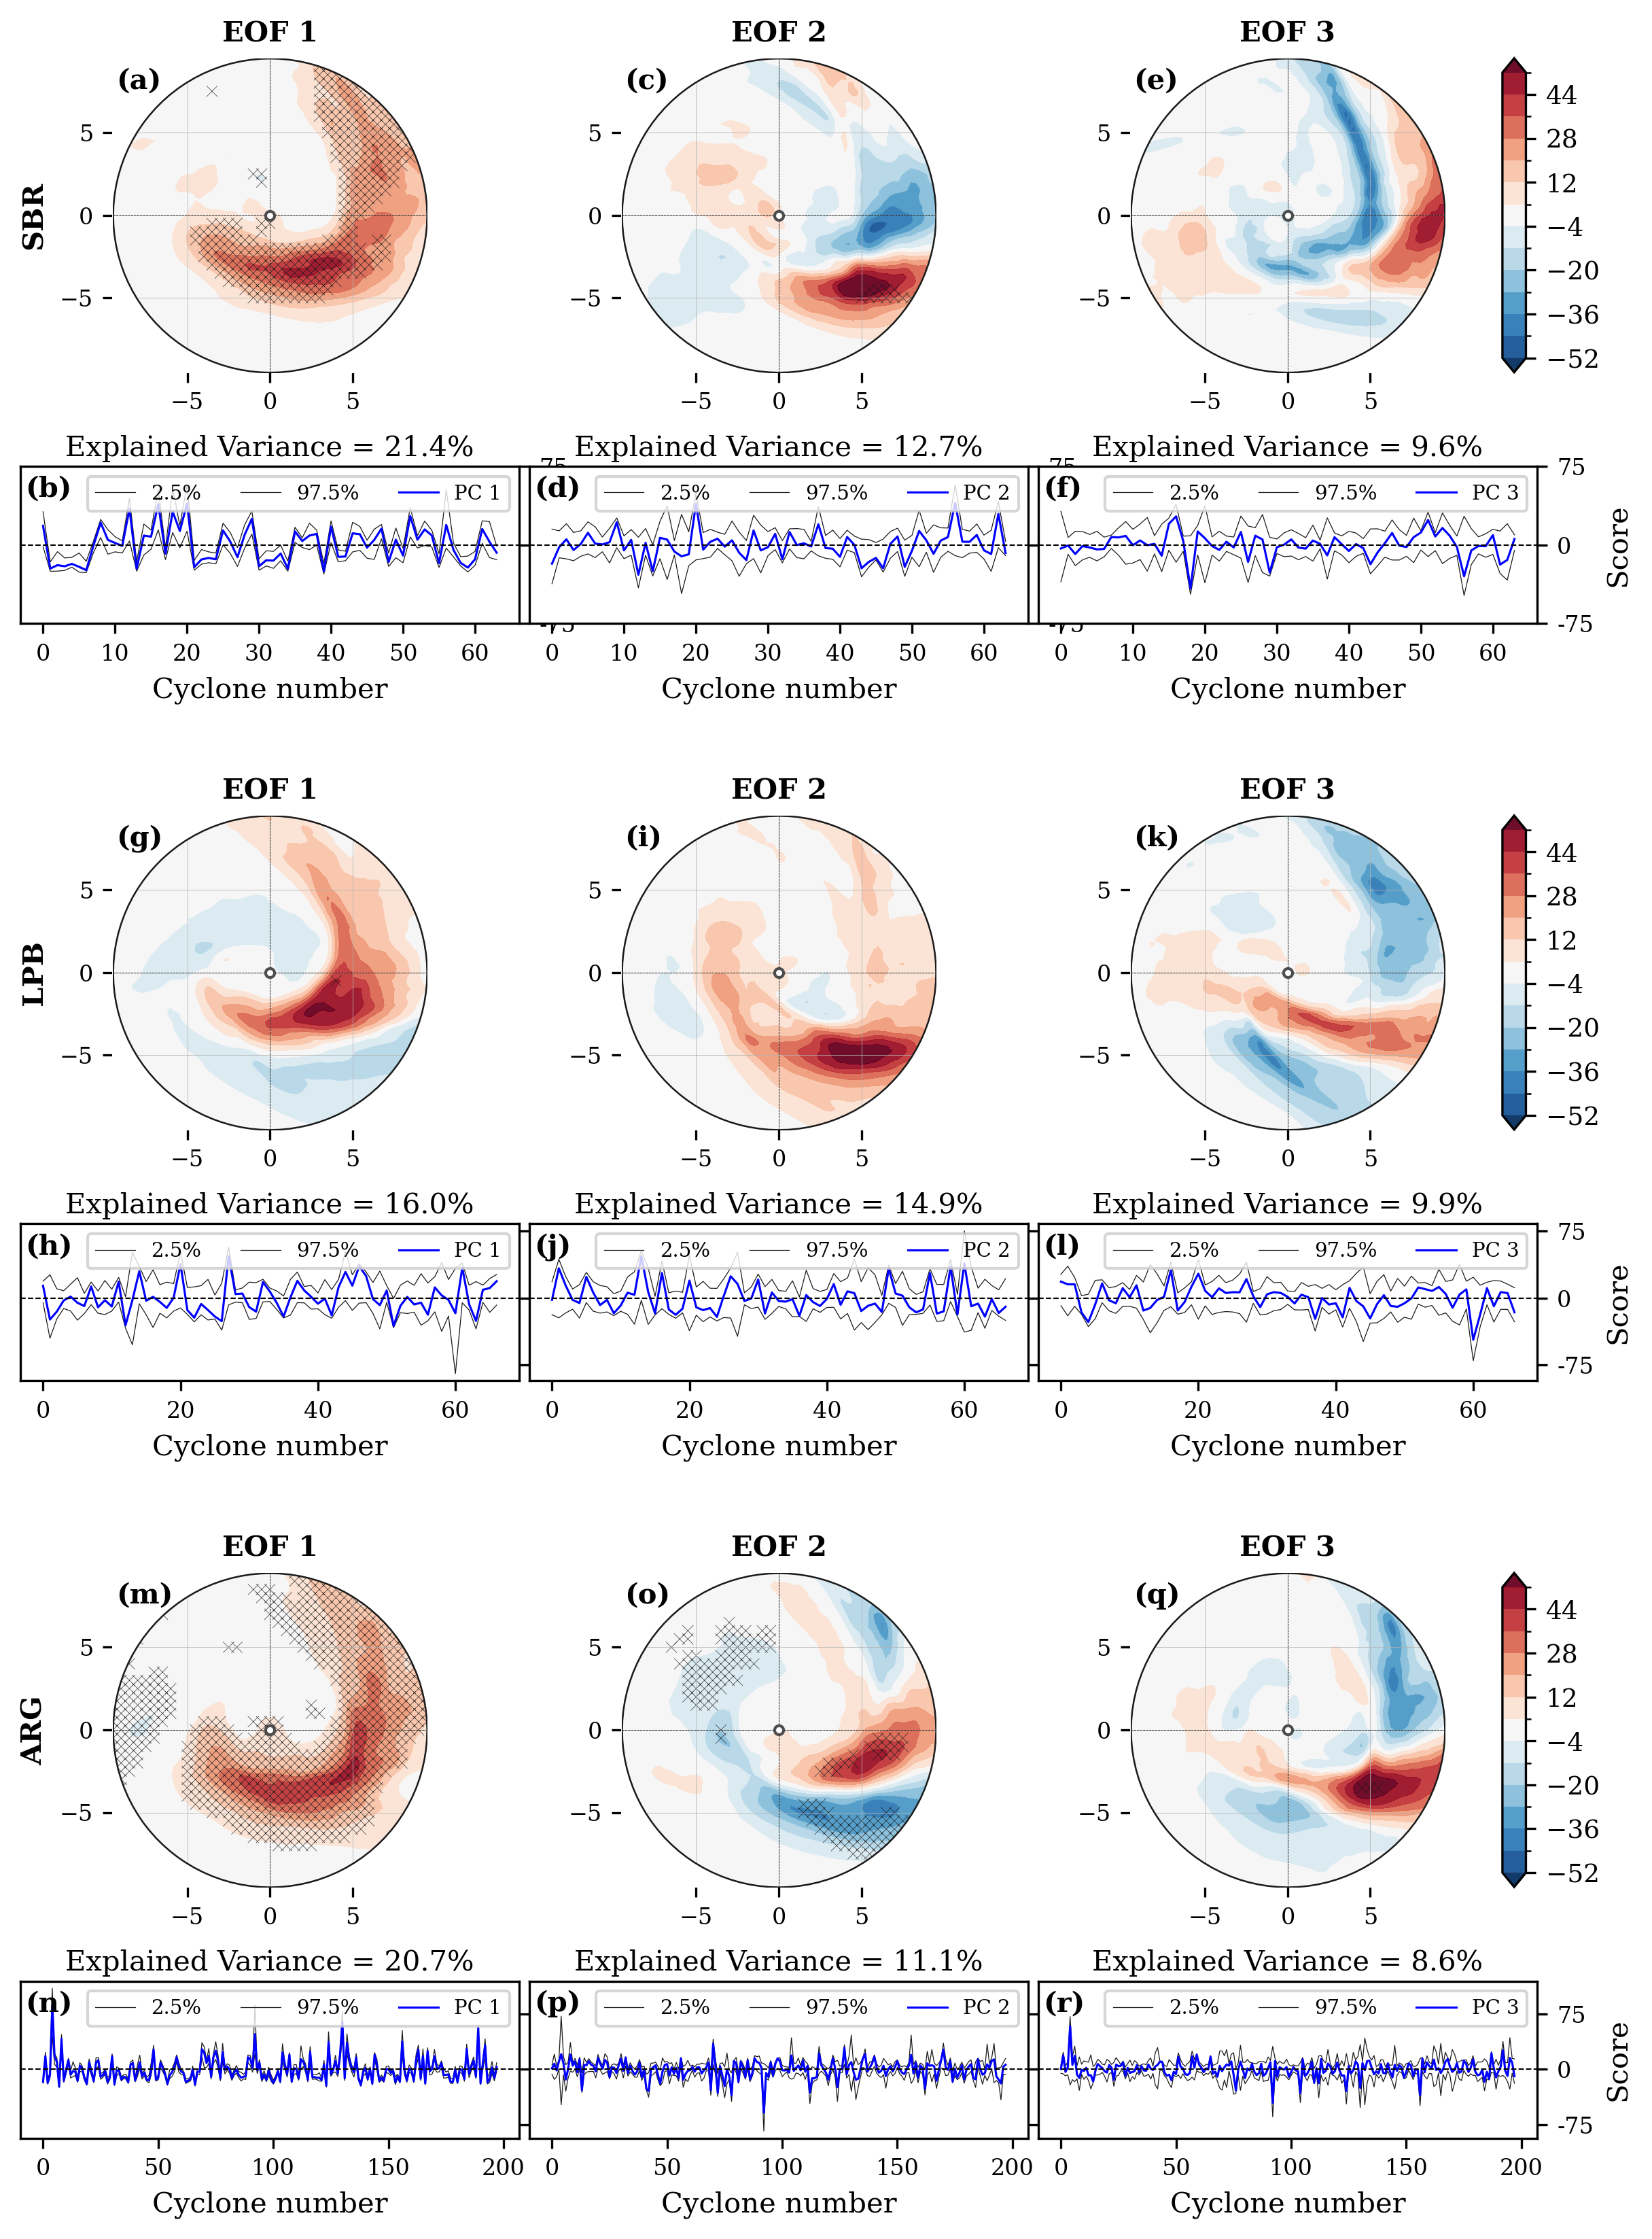
\includegraphics[width=\textwidth]{images/tp/xeof_p90_tp_mature.png}
\caption[Significancia espacial de los EOFs en fase de madurez - Subconjunto p90 (tp)]{Descomposición EOF de la precipitación total para el subconjunto extremo (p90) en fase de madurez. La disposición de paneles es idéntica a la Figura~\ref{fig:xeof_madurez_global_tp}.}
\label{fig:xeof_madurez_p90_tp}
\end{figure}

La Figura~\ref{fig:xeof_madurez_global_tp} evidencia que, para la Población Global en fase de madurez, las áreas de significancia estadística del EOF1 aparecen confinadas al sector oriental del dominio, coherentes con el forzante del Cinturón Transportador Cálido documentado previamente. Sin embargo, a diferencia del campo de viento donde la significancia abarcaba dominios extensos y contiguos, aquí las zonas significativas se presentan fragmentadas, con manchas aisladas de achurado que no forman un patrón geométrico continuo. Este aspecto visual refleja directamente la naturaleza inherentemente discontinua de la precipitación, donde la convección embebida y los frentes estrechos generan señales espaciales localizadas pero no necesariamente coherentes a escala sinóptica completa. Las series temporales asociadas (paneles b, d, f) muestran que las fluctuaciones de PC2 y PC3 permanecen mayoritariamente dentro de los límites de confianza del 95\%, indicando que los modos secundarios capturan variabilidad de menor relevancia física en la climatología general.

Por el contrario, la Figura~\ref{fig:xeof_madurez_p90_tp} revela una transformación cualitativa en el patrón de significancia. En el subconjunto extremo, y consistente con el salto en la varianza explicada documentado en la Sección~\ref{subsec:var_exp_tp}, el EOF1 concentra sus áreas significativas en una configuración curvada que abarca el sector sureste y sur del dominio, trazando la geometría de la banda enroscada. A diferencia de la población global, aquí el achurado forma un arco continuo y denso que bordea el cuadrante central, indicando que la señal física es estadísticamente robusta en toda la extensión de la estructura periférica. Notablemente, las series de PC2 y PC3 muestran amplitudes que en ciertos periodos alcanzan o superan los límites de confianza bootstrap, sugiriendo que incluso la variabilidad secundaria adquiere relevancia física durante la transición hacia el decaimiento en sistemas severos.

Esta diferencia en la distribución espacial de la significancia tiene implicaciones operativas directas para la predictibilidad de los impactos. En la Población Global, la fragmentación de la significancia indica que la ubicación exacta de los máximos de precipitación presenta mayor incertidumbre espacial, respondiendo a la variabilidad inherente de los procesos convectivos transitorios. Sin embargo, en los sistemas extremos durante el decaimiento, la concentración de significancia en la banda enroscada periférica representa una ganancia de predictibilidad geométrica: la huella pluviométrica se ancla en una estructura espacialmente coherente y estadísticamente replicable. Esto contrasta marcadamente con el comportamiento observado en el viento, donde la contracción de la significancia hacia el núcleo en sistemas extremos indicaba una pérdida de predictibilidad para los flancos exteriores. En el caso de la precipitación, la organización ocluida genera una firma predecible para la alerta temprana, concentrando el peligro hidrológico en sectores periféricos bien delimitados durante la fase final del ciclo de vida.
%%%%
%%%%%%
%%%%
%%
% ==============================================================================
\section{Dinámica temporal: Componentes principales (PC1)}\label{sec:dinamica_pc1_tp}
% ==============================================================================

La fragmentación de la varianza documentada en la fase de madurez y su transformación hacia la coherencia en el decaimiento tienen su contraparte temporal en el comportamiento estadístico de las Componentes Principales. El contraste entre la Población Global y los ciclones extremos revela aquí una dinámica inversa a la observada en el viento: mientras el campo cinemático mostraba un fortalecimiento progresivo de la correlación hasta la madurez seguido de un colapso en los sistemas p90, el campo pluviométrico exhibe una firma correlacional invertida y distribuciones de probabilidad marcadamente leptocúrticas en todos los estratos.

% 
\subsection{Población Global}\label{subsubsec:pc1_global_tp}
% Acoplamiento débil y distribuciones con cola
% TABLA 1: MOMENTOS ESTADÍSTICOS - POBLACIÓN GLOBAL
\input{tabelas_es/tab_momentos_global_tp.tex}

% TABLA 2: CORRELACIONES - POBLACIÓN GLOBAL
\input{tabelas_es/tab_corr_global_tp.tex}

Las Tablas~\ref{tab:momentos_global_tp} y~\ref{tab:corr_global_tp} documentan las propiedades estadísticas de la primera Componente Principal (PC1) para la Población Global. La primera tabla presenta los momentos de orden superior (sesgo $\gamma_1$ y curtosis $\gamma_2$) que caracterizan la forma de la distribución de amplitudes del modo espacial dominante, mientras que la segunda tabla muestra los coeficientes de correlación de Pearson entre la PC1 y el mínimo de vorticidad relativa a 850 hPa ($\zeta_{850}^{min}$) alcanzado por cada ciclón. Los valores se desagregan por región de ciclogénesis y fase evolutiva, permitiendo evaluar tanto la estructura interna de la variabilidad como su relación con la intensidad dinámica del sistema.

El análisis de los momentos estadísticos revela una característica distintiva del campo pluviométrico: la presencia persistente de distribuciones con colas pesadas (leptocurtosis positiva) a lo largo de todo el ciclo de vida. A diferencia del viento, donde la curtosis evolucionaba hacia valores cercanos a cero o negativos durante la madurez, en la precipitación se observan valores de $\gamma_2$ consistentemente positivos. En SBR estos valores oscilan entre $+0.87$ en intensificación y $+2.18$ en decaimiento; LPB exhibe curtosis pronunciada en incipiencia ($+2.85$) y particularmente en decaimiento ($+6.02$); mientras que ARG presenta los valores más extremos, con curtosis superiores a $+9$ tanto en incipiencia como en decaimiento. El sesgo positivo persistente ($\gamma_1 > +0.8$ en la mayoría de los casos) indica que la distribución de amplitudes presenta una cola extendida hacia valores altos, reflejando la presencia de eventos con anomalías pluviométricas excepcionalmente intensas respecto al patrón medio.

El examen de las correlaciones entre PC1 y vorticidad revela un desacoplamiento progresivo entre la estructura espacial de la precipitación y la intensidad rotacional del vórtice durante la madurez en las regiones oceánicas. En SBR, la correlación negativa moderada durante las fases iniciales ($\rho \approx -0.52$) invierte su signo en la madurez ($\rho = +0.17$, significativo) y decaimiento ($\rho = +0.19$, significativo), indicando que los ciclones con mayor vorticidad tienden a presentar menores amplitudes en el modo dominante de precipitación durante estas etapas. LPB muestra un patrón similar: correlaciones negativas significativas durante el desarrollo ($\rho = -0.49$ en incipiencia, $-0.59$ en intensificación) que colapsan hacia valores no significativos en madurez ($\rho = -0.04$, $p = 0.26$) y decaimiento ($\rho = -0.07$, $p = 0.07$). En contraste, ARG mantiene correlaciones negativas estadísticamente significativas durante todo el ciclo, aunque con debilitamiento progresivo (de $-0.51$ en incipiencia a $-0.25$ en decaimiento).

Este comportamiento correlacional refleja procesos físicos diferenciados en la evolución del ciclo de vida. El cambio de signo observado en SBR y el colapso en LPB durante la madurez responden a la divergencia entre intensidad dinámica y actividad convectiva documentada en las distribuciones de probabilidad. En estas regiones, los sistemas que alcanzan valores extremos de vorticidad son precisamente los que desarrollan oclusiones más completas y rápidas, donde la intrusión seca suprime la convección profunda en el dominio central lagrangiano. Por ello, la PC1, que captura la variación de la huella pluviométrica en el dominio de análisis, ya no escala positivamente con la profundidad del vórtice: los ciclones más intensos dinámicamente presentan anomalías menores en el modo de precipitación porque su núcleo se ha secado. En ARG, la oclusión es más lenta y el agotamiento de humedad más gradual debido a la modulación orográfica, lo que permite mantener un acoplamiento residual entre vorticidad y precipitación durante más tiempo.

La variabilidad temporal de estas series de PC1, manifestada en los picos de amplitud inter-anual, responde a fluctuaciones de gran escala en la circulación hemisférica. Las oscilaciones de baja frecuencia en la baroclinicidad del Hemisferio Sur, analizadas por \citet{machado2020influence}, modulan la eficiencia de los sistemas ciclónicos para condensar vapor de agua. Durante periodos de mayor inestabilidad baroclínica, caracterizados por cizalladura vertical intensificada y gradientes térmicos elevados en el espesor troposférico, la PC1 exhibe amplitudes superiores a la media, reflejando condiciones favorables para la generación de anomalías pluviométricas extremas. Complementariamente, \citet{simmonds2000variability} documentan ciclos temporales en la profundidad y extensión de los ciclones extratropicales del Hemisferio Sur, sugiriendo que los picos de la serie temporal de PC1 capturan ventanas de mayor actividad ciclogenética donde la convergencia de niveles bajos se intensifica, forzando tasas de condensación superiores a la climatología estándar en los estratos moderados y extremos de la población.

% 
\subsection{Subconjunto Extremo (p90)}\label{subsubsec:pc1_p90_tp}
%Leptocurtosis extrema, colapso correlacional y asimetría regional
% TABLA 3: MOMENTOS ESTADÍSTICOS - P90
\input{tabelas_es/tab_momentos_p90_tp.tex}
% TABLA 4: CORRELACIONES - P90
\input{tabelas_es/tab_corr_p90_tp.tex}

Las Tablas~\ref{tab:momentos_p90_tp} y~\ref{tab:corr_p90_tp} documentan las propiedades estadísticas de la PC1 para el estrato de ciclones extremos. La primera tabla presenta la evolución de los momentos de orden superior (sesgo y curtosis) a través de las fases del ciclo de vida, mientras que la segunda tabla registra los coeficientes de correlación entre la amplitud del primer modo y la vorticidad mínima del sistema. La comparación con las tablas correspondientes de la Población Global revela una dinámica cualitativamente distinta: en lugar de la leptocurtosis persistente observada previamente, aquí se documenta una evolución no monotónica hacia valores extremos en el decaimiento, acompañada de un colapso sistemático de las correlaciones durante la fase de madurez en las regiones oceánicas.

El análisis de las distribuciones de probabilidad revela una heterogeneización dramática del comportamiento estadístico. En SBR se observa leptocurtosis marcada en las fases iniciales ($\gamma_2 = +3.48$ en incipiencia, $+1.67$ en intensificación), seguida de un colapso hacia una distribución cuasi-normal en la madurez ($\gamma_2 = -0.67$) y una explosión leptocúrtica en el decaimiento ($\gamma_2 = +19.77$, $\gamma_1 = +4.02$). LPB reproduce este patrón con valores aún más extremos: curtosis de $+4.52$ en incipiencia, evolución hacia simetría en madurez ($\gamma_2 = +0.16$), y valores superiores a $+23$ en decaimiento. ARG presenta la curtosis más elevada del conjunto en fase incipiente ($+30.88$), manteniendo valores positivos extremos durante todo el ciclo. Simultáneamente, las correlaciones con la vorticidad exhiben un colapso estadístico durante la madurez en SBR ($\rho = -0.17$, no significativo) y LPB ($\rho = -0.03$, $p = 0.80$), recuperándose parcialmente en el decaimiento ($-0.34$ y $-0.50$ respectivamente), mientras que ARG mantiene valores negativos significativos aunque atenuados ($-0.24$ en madurez).

La variabilidad temporal de estas series, manifestada en los pulsos de alta amplitud observados en las series de PC1, responde a las escalas características de los extremos ciclónicos. Como evidencian \citet{chen2025characteristics}, los eventos de precipitación extrema asociados a ciclones extratropicales están dinámicamente constreñidos a periodos cortos, con escalas temporales del orden de 2 a 3 horas para las tasas máximas de condensación. Esta limitación temporal explica las fluctuaciones inter-diarias violentas observadas en las series de PC1: los picos pluviométricos de máxima intensidad representan inyecciones fugaces de ascensos térmicos embebidos en el ciclo de vida sinóptico de los ciclones, generando la cola pesada que caracteriza a las distribuciones del estrato p90.

El colapso correlacional durante la madurez en SBR y LPB constituye el correlato temporal del desacoplamiento espacial documentado en los análisis de PDF y KDE. Cuando los vórtices extremos alcanzan su máxima profundidad dinámica, la precipitación en el dominio lagrangiano deja de ser gobernada por la intensidad rotacional del sistema para depender de la geometría específica de la oclusión. La posición de la banda enroscada respecto al centro del dominio determina la presencia o ausencia de anomalías positivas en la PC1, introduciendo variabilidad que no correlaciona linealmente con la vorticidad. Esto explica la evolución hacia la normalidad estadística en la madurez seguida de la explosión leptocúrtica en el decaimiento: a medida que los sistemas se disipan, algunos retienen la banda enroscada dentro del dominio (generando la cola positiva extrema), mientras otros la han desplazado hacia el exterior.

Este desacoplamiento obedece a una reestructuración termodinámica impulsada por retroalimentaciones locales de mesoescala. Durante el análisis del evento severo Raoni en el Atlántico Sur, \citet{reboita2022from} documentan cómo los flujos turbulentos de superficie alimentan convección vigorosa que redistribuye la vorticidad potencial mediante liberación masiva de calor latente. Este calentamiento diabático reduce la cizalladura vertical y consolida la seclusión cálida, desacoplando la dinámica de la precipitación periférica de las fluctuaciones lineales del gradiente sinóptico de fondo, otorgándole a los ciclones maduros una evolución cuasi-independiente respecto a la intensidad del vórtice.

La alteración de la estructura vertical de la vorticidad potencial durante la madurez rompe la linealidad entre campos de superficie y dinámica de gran escala. Según \citet{crespo2021potential}, la evolución de los ciclones en el este de Sudamérica está ligada a la interacción entre anomalías de vorticidad potencial en la alta troposfera y el calentamiento diabático en niveles bajos. En sistemas extremos, la liberación masiva de calor latente asociada a las precipitaciones enroscadas genera profundas anomalías de vorticidad potencial en la baja troposfera que dominan la circulación local, rompiendo la relación lineal con el gradiente de presión de fondo y propiciando la bifurcación estructural observada en las series temporales.

La persistencia de correlaciones significativas en ARG durante toda la evolución refleja una dinámica de oclusión diferenciada. En esta región, los ciclones desarrollan oclusiones más lentas y heterogéneas, con intrusión seca menos violenta que en las regiones oceánicas. La modulación orográfica de la cordillera de los Andes y el control de la humedad por advección zonal, en lugar de intercambio oceánico, generan un acoplamiento más persistente entre vorticidad y precipitación, aunque atenuado respecto a las fases iniciales. Esto explica por qué en ARG la PC1 nunca pierde completamente su correlación con la intensidad dinámica, manteniendo valores significativos incluso durante la madurez.

Estos resultados demuestran que el campo pluviométrico extremo es estructuralmente más complejo que el cinemático. La combinación de distribuciones con colas pesadas variables, correlaciones que colapsan y recuperan, y diferencias regionales marcadas indica que parametrizar la precipitación asociada a eventos severos utilizando únicamente la vorticidad o la presión mínima resulta inadecuado, particularmente durante la fase crítica de madurez en las regiones oceánicas donde el desacoplamiento es más pronunciado.
%%
%%%%
%%%%%%
%%%%
%%

% ==============================================================================
\section{Síntesis}\label{sec:sintesis_tp}
% ==============================================================================

El análisis del campo de precipitación total revela una arquitectura hidrometeorológica que evoluciona desde un régimen de dispersión frontal hacia uno de concentración ocluida, dependiendo críticamente de la intensidad dinámica del sistema. En la población global, la precipitación se organiza como una respuesta asimétrica al forzante del Cinturón Transportador Cálido: las distribuciones de probabilidad exhiben colas pesadas persistentes (sesgo positivo y leptocurtosis), los máximos se concentran en el cuadrante oriental del dominio lagrangiano, y la varianza espacial se distribuye entre múltiples modos sin que el EOF1 domine abrumadoramente. Esta configuración refleja que, en el régimen promedio, la lluvia está gobernada por la disponibilidad de humedad ambiental y la convergencia frontal transitoria del WCB, sin una dependencia lineal de la profundidad rotacional del vórtice, como confirman las correlaciones débiles o inexistentes entre PC1 y vorticidad durante la madurez en SBR y LPB.

En contraste, los sistemas extremos (p90) exhiben una arquitectura pluviométrica cualitativamente diferente que emerge de la transición hacia la oclusión severa. La reorganización espacial observada en el KDE y el salto en la varianza explicada por el EOF1 (del 11--16\% típico al 36,5\% en LPB durante el decaimiento) responden primariamente al proceso de oclusión al estilo Shapiro-Keyser. La intrusión seca profunda aniquila la convección en el núcleo central y confina la humedad remanente en una banda periférica enroscada (*wrap-around precipitation*) topológicamente coherente \citep{schultz2021antecedents}. Este proceso genera el colapso de las PDF hacia modas de baja precipitación central simultáneo al pico de vientos destructivos, confirmando el desacople temporal entre forzantes cinemático e hidrológico en los eventos más severos.

La superposición de los campos de viento y precipitación en los sistemas extremos evidencia geométricamente el desacople espacial de los peligros. Mientras los vientos máximos se concentran en el cuadrante noroeste asociados a la cinta transportadora fría, los máximos pluviométricos remanentes se organizan en una herradura sólida en el sureste y sur, orbitando el margen de la intrusión seca. Esta configuración opera bajo el marco conceptual de eventos compuestos (*compound events*), donde los peligros extremos surgen de la combinación de múltiples procesos físicos interactuando a diferentes escalas \citep{zscheischler2018future}. En el Atlántico Sudoccidental, esto implica que las amenazas más severas por inundaciones relámpago ocurrirán preferentemente durante las etapas de génesis e intensificación cuando el acceso a la humedad tropical es activo.

Las diferencias regionales modulan esta arquitectura general mediante la interacción con las condiciones de superficie. En SE-BR y LPB, los flujos de calor latente oceánico y el chorro de capas bajas favorecen el desarrollo del desacople más pronunciado entre vorticidad y precipitación, mientras que en ARG la modulación orográfica y oclusiones más lentas generan un régimen de transición más gradual entre dinámica y humedad, como refleja la persistencia de correlaciones significativas en esta región \citep{marrafon2022classificacao}. Esta multiplicidad de vías evolutivas, donde la plasticidad termodinámica del núcleo determina la organización espacial final, explica la coexistencia de distribuciones heterogéneas entre regiones a lo largo del ciclo de vida.

El establecimiento de esta base hidrometeorológica —en particular la demostración estadística del desacople espaciotemporal entre viento y lluvia en eventos severos— provee el cimiento teórico para el análisis combinado mediante Funciones Ortogonales Empíricas Multivariadas (MEOF) en el capítulo siguiente, donde se explorará explícitamente la covarianza conjunta de ambos campos destructivos y sus implicaciones para la evaluación integrada del riesgo.
%%
%%%%
%%%%%%
%%%%
%%
